%----------------------------------------------
\documentclass[12pt,a4paper]{report}
\RequirePackage[english,russian]{babel}
\usepackage[utf8x]{inputenc}
\usepackage{amsmath}
\usepackage{amsfonts}
\usepackage{amssymb}
\RequirePackage{graphicx}
\usepackage{listings}
\lstset{language=C++, texcl=true, frame=lines, basicstyle=\ttfamily}  % latex в комментариях 
\usepackage{natbib}
%-----------------------------------------------
\providecommand{\abs}[1]{\lvert#1\rvert}
\providecommand{\norm}[1]{\lVert#1\rVert}
\providecommand{\frqt}[1]{\guillemotleft#1\guillemotright}
\providecommand{\bvec}[1]{\mathbf{#1}}
%-----------------------------------------------

%- additional tuning ---------------------------
\graphicspath{{images/}} % путь к рисункам
%-----------------------------------------------

\begin{document}

%-----------------------------------------------
%\title{Виртуальный полигон для исследования морских объектов в экстремальных условиях эксплуатации}
%\author{А. А. Безгодов}
%\date{\today}
%\maketitle
%\setcounter{page}{3}
%-----------------------------------------------


%\begin{titlepage}
\begin{center}

Санкт-Петербургский Государственный Университет Информационных Технологий, Механики и Оптики

\begin{flushright}
\textit{\textbf{На правах рукописи}}
\end{flushright}

\vspace*{0.5in}

\vspace{1.0in}
{\large А.А. Безгодов}
\vspace{0.25in}

{\large ВИРТУАЛЬНЫЙ ПОЛИГОН ДЛЯ ИССЛЕДОВАНИЯ МОРСКИХ ОБЪЕКТОВ В ЭКСТРЕМАЛЬНЫХ УСЛОВИЯХ ЭКСПЛУАТАЦИИ}
\vspace{0.5in}

Специальность: 05.13.18 --- Математическое моделирование, численные методы и комплексы программ
\vspace{0.25in}

Диссертация на соискание ученой степени  \linebreak
%\textsl{кандидата технических наук}
кандидата технических наук
\vspace{0.5in}

\begin{flushright}
Научный руководитель \linebreak
Доктор технических наук, \linebreak
А.В. Бухановский \linebreak
\end{flushright}

\vspace{1.0in}
Санкт-Петербург  \linebreak
2011



\end{center}
\end{titlepage}

%
%\tableofcontents
%
%\chapter*{Введение}
\addcontentsline{toc}{chapter}{Введение}

Бла-бла-бла
%
%\chapter{Технология виртуальных полигонов для моделирования сложных технических объектов и систем}


%\section{Технология виртуальных полигонов}
\label{ch1_1_1}

Специфика исследовательского проектирования морских объектов состоит в неопределенности и неполноте информации об их поведении в экстремальных ситуациях, совокупно вызванных воздействием внешней среды, инициируемых им опасных ситуаций (например, интенсивным обледенением) и внутренних дестабилизирующих факторов (смещения груза, затопления отсеков и пр.). При этом развитие аварийной ситуации происходит по различным сценариям, которые не могут быть в общем случае сведены к ограниченному набору типовых случаев. Однако ретроспективный анализ гибели судов позволяет выделить условия, способствующие возникновению аварийных ситуаций. При движении судна лагом к волне выделяют такие ситуации, как воздействие на судно ветрового шквала в условиях сильной качки, потеря остойчивости по причине затопления палубного колодца, а также ударное воздействие гребня разрушающейся волны. Напротив, при попутном волнении начинают играть роль совершенно другие критические факторы, а именно: параметрический резонанс бортовых колебаний, потеря управляемости на гребне волны, захват судна волной (брочинг). В свою очередь, развитие каждой из вышеперечисленных ситуаций может усложняться за счет внутренних факторов (смещение навалочного груза, затопление отсеков, интенсивное обледенение и пр.). Неоднозначность условий, приводящих к возникновению аварийных ситуаций, в данном случае затрудняет обоснование оптимальных проектных характеристик судна формальными методами и приводит к необходимости использования методов виртуального моделирования. Иными словами, основным инструментом поддержки принятия решений в процессе исследовательского проектирования становятся численные модели динамики морских объектов \citep{nechaev_ai}, позволяющие количественно воспроизвести их поведение под воздействием реалистичных внешних возмущений.

Таким образом, единственным способом моделирования рассматриваемых ситуаций является программное численное моделирование. В связи с этим вводится понятие виртуального полигона (Virtual test bed).
Виртуальный полигон – это программно-аппаратное средство, которое поддерживает виртуальное проектирование, анализ и прототипирование различных систем \citep{vtb_ship_ee} \citep{vtb_ILRO}. 

Виртуальный полигон должен удовлетворять следующим требованиями:
\begin{itemize}
	\item 	Реальное время выполнения (в идеале --- «сверхреальное»). «Сверхреальное» 
			время выполнения позволит перебирать несколько вариантов параллельно, что может быть полезно для предсказания поведения реальных объектов, а также производить массовую статистическую выборку.
	\item 	Интерактивность. В данном случае под интерактивностью подразумевается 
			возможность изменения параметров моделируемых объектов и получения 
			ответной реакции в реальном времени.
	\item 	Гибкость. Виртуальный полигон должен предоставлять набор конструктивных 
			и вспомогательных объектов для формирования задачи моделирования.  
			При этом объекты могут быть как конструктивными, так и вспомогательными. 
			Конструктивные отвечают за определение и формирование поведения и свойств 
			реального объекта, а вспомогательные позволяет формировать сценарии 
			модельных процессов и обработки результатов.
	% \item Возможность самонастройки и самоподстройки. 
	% Виртуальный полигон должен обеспечивать возможность гибкого 
	\item 	Возможность расширения: возможность добавления новых явлений, свойств и объектов.
\end{itemize}

Анализ задач моделирования динамики судна \citep{nechaev_ai}, а также виртуальных полигонов, использующихся в других научных и инженерных областях показал, что в состав виртуального полигона должны входить следующие компоненты:
\begin{itemize}
	\item   Подсистема человеко-машинного взаимодействия, в состав которой входят:
		\begin{itemize}
		\item 	Подсистема визуализации и отображения данных, 
				которая отвечает за отображение текстовой информации, 
				построения диаграмм а также двумерной, трехмерной и 
				стерео-визуализации моделируемого процесса.
		\item 	Подсистема ввода, которая может включать разнообразные 
				устройства ввода, начиная от простейшего текстового 
				интерфейса терминального типа и заканчивая интерфейсами 
				основанными на захвате движения.
		\end{itemize}
	\item	одсистема моделирования --- является центральной 
			частью виртуального полигона и отвечает за расчет пареметров 
			моделируемого объекта в каждый момент времени. Подсистема 
			моделирования может быть как монолитной, так и композитной. 
			В последнем случае, каждая компонента подсистемы моделирования 
			выполняет свою задачу и обменивается данными с другими компонентами.
	\item	Подсистема сценариев --- подсистема, которая отвечает за 
			формирование последовательностей, условий и дополнительных 
			действий, выполняемых в процессе моделирования.
\end{itemize}

Подсистемы виртуального полигона могут быть либо собраны в один програмный пакет, запускаемый на персональной ЭВМ так и сформированны в распределенный программно-аппаратный комплекс, который может состоять из:
\begin{itemize}
	\item 	Вычислительных серверов, кластеров, на которых 
			могут быть развернуты компоненты подсистемы моделирования.
	\item 	Графических станции, которые формируют изображение 
			целиком или по фрагментами. Разные графические могут 
			визуализировать моделируемый процесс с разных точек, 
			в разных масштабах и режимах отображения.
	\item 	Компонент ввода, которые могут включать в себя клавиатуры, 
			мыши, сенсорные панели, системы захвата движения, нейро-интерфейсы и т.п.
\end{itemize}






%\section{Математические модели динамики внешней среды}

Основная задача математического моделирования динамики судна связана с обеспечением устойчивости его движения и формулируется как определение области в пространстве состояний судна, соответствующей требованиям эксплуатации, поиск границы этой области и связь параметров судна с критическими значениями параметров действующих возмущений \citep{dk1}. Исследование в такой постановке может быть выполнено только на основе анализа движения судна, находящегося под действием вызванных ветром и волнением сил. По этой причине для решения задачи построения модели динамики судна под воздействием внешней среды в экстремальных условиях эксплуатации необходимо разделить собственно математические (имитационные) модели изменчивости внешней среды и модели динамики морского объекта, находящегося в ней.

Непрерывный рост численности судов мирового флота, а также бурное освоение шельфовой зоны требуют не только умения предсказывать неблагоприятные погодные условия с той или иной заблаговременностью, но и определять количественные характеристики морских явлений редкой повторяемости, характеризующих экстремальную динамику внешней среды. К ним относятся скорость ветра, морское волнение, течения и уровень моря, а также их сочетания, возможные один раз в 100 или даже 1000 лет. Современная концепция получения информации о состоянии Мирового океана предполагает модельный подход на базе гидродинамического и статистического моделирования ветра, волнения, течений и уровня моря \citep{dk2}.

В инженерной практике экстремальные гидрометеорологические явления характеризуются расчетными сочетаниями скоростей ветра, параметров волнения, скоростей течений и уровня моря, возможными 1 раз в $T$ лет, где $T$ соответствует классу сооружения. Современная концепция получения информации об экстремальных гидрометеорологических явлениях основана на синтетическом подходе: на основе упорядоченных массивов метеорологической информации за несколько десятков лет выполняется гидродинамическое моделирование полей течений, морского волнения и уровня моря. Эти данные используются для идентификации стохастической модели, на основе которой выполняется экстраполяция расчетных характеристик на период повторяемости $T$. 

В рамках концепции \citep{dk3} основным источником данных об океанографических процессах (волнении, уровне, течениях) является сертифицированная (или, в метрологической практике – аттестованная) гидродинамическая модель динамики океана. По ней выполняются расчеты за непрерывный исторический период, обеспеченный данными наблюдений за атмосферными процессами (давлением, ветром и температурой воздуха). Гидродинамическая модель может быть интерпретирована как виртуальная измерительная система, верифицированная на основе разрозненных данных измерений, уже имеющихся в данном районе Мирового океана. Такой подход позволяет, используя данные реанализа метеорологических полей, получать информационные массивы океанографических характеристик непрерывной продолжительностью несколько десятков лет \citep{dk4}. Для статистического оценивания экстремальных характеристик, возникающих с определенной вероятностью, используется система стохастических моделей, описывающих совместную многомасштабную изменчивость пространственно-временных полей океанографических характеристик. Это дает возможность методом Монте-Карло воспроизвести ансамбль их реализаций, таким образом экстраполируя значения экстремумов на заданный временной интервал.

Следует отметить, что экстремальность гидрометеорологического явления по отношению к конкретному объекту определяется интегральной совокупностью всех факторов путем рассмотрения функций риска, специфичных для определенных классов морских объектов и сооружений. Это позволяет интерпретировать экстремальные гидрометеорологические явления не только в терминах скалярных характеристик (высоты волны, периода и пр.), а непосредственно в рамках формализма многомерных экстремумов.

Для имитационного моделирования конкретных воздействий на морские объекты и сооружения применяется иерархия моделей, позволяющая адекватно учесть многомасштабную изменчивость, обусловленную прохождением штормов. Так, для воспроизведения полей волнения в мелкомасштабном (секунды--часы) диапазоне изменчивости конкурентно (в зависимости от формы спектра) используются модели в форме полевой авторегрессии \citep{dk6} или в форме ортогональных разложений со случайными коэффициентами \citep{dk7}, в том числе с учетом нелинейности волнового профиля \citep{dk8}. Учет штормовой активности, в свою очередь, в диапазоне синоптической изменчивости осуществляется двумя альтернативными путями – посредством модели авторегрессии-скользящего среднего \citep{dk9} в синоптическом диапазоне (в терминах характерной высоты волны) или в терминах импульсной модели пространственно-временного поля в рамках лагранжева формализма \citep{dk10}. Учет климатической неоднородности, в свою очередь, требует применения другого класса моделей на основе ортогональных разложений по каноническому базису (естественные ортогональные функции) \citep{dk11}.

Для стохастического моделирования полей морского волнения может использоваться модель, основанная на использовании процессов авторегрессии-скользящего среднего \citep{p295I_31} в фиксированной точке пространства. Эта модель основывается на представлении процесса волнения как решения линейного дифференциального уравнения N-го порядка с постоянными коэффициентами и случайным входным сигналом.

Модель авто\-регрессии-скользящего среднего при высоком порядке по каждой из координат в рамках корреляционной теории является эквивалентной другой форме записи пространственно-временного случайного гауссова поля --- линейной модели Лонге-Хиггинса \citep{p295I_45}, котоое является формой разложения в дискретный ряд Фурье \citep{krogstad89}.

Для идентификации параметров моделей волнения необходимо знать корреляционную функцию или функцию спектральной плотности волновой поверхности. Спектральная плотность (или просто спектр) отражает свойства поля волнения при неизменных внешних факторах, как квазистационарного и квазиоднородного процесса. Изменения условий волнообразования связаны с прохождением барических образований (синоптическая изменчивость), годовой ритмикой (сезонная изменчивость) и долгопериодными вариациями циркуляционных процессов (межгодовая изменчивость), что позволяет определить волновой климат (или режим волнения) как ансамбль состояний волновой поверхности с учетом указанной изменчивости и описать его в терминах режимных статистических характеристик. Набор параметров из ансамбля промежутков квазистационарности характеризует волновой климат \citep{dk4}.

В целом волновой климат описывается ансамблем реализаций спектров за временной интервал, характеризуемый обычно несколькими десятками лет, в каждой точке  акватории. В силу такого подхода в качестве отдельных сценариев состояний моря выступают так называемые климатические спектры. Климатический спектр — это конкретный спектр, имеющий определенную вероятность (повторяемость появления в климатическом ансамбле) и отражающий ситуации, характерные для некоторого набора условий волнообразования \citep{dk4}. Для определения климатических спектров заданной повторяемости используются методы класса Монте-Карло \citep{dk8} или более сложные методы на основе многопараметрической оптимизации  \citep{dk5}.

Для отдельных задач моделирования внешних воздействий в режиме мелкомасштабной изменчивости используются физико-статистические методы. В частности, это связано с ситуациями, когда гидродинамические характеристики отдельной волны имеют определяющее влияние на объект, а априори восстановить ее профиль не представляется возможным. Такой подход характерен для моделирования волн-убийц и их воздействия на морские объекты и сооружения \citep{dk12}\citep{dk13}. Однако его применение далеко не всегда оправдано в силу ресурсоемкости вычислений.

Таким образом, рассмотренные модели позволяют воспроизводить изменчивость внешних возмущений, воздействующих на морской объект, в соответствии с их климатической повторяемостью для характерного района Мирового океана. Это дает возможность их использования в качестве входных данных для моделирования динамики морских объектов.
%\section{Математические модели динамики морских объектов}

Основными целями изучения динамики корабля под воздействием внешних условий является обеспечение корабля качествами, в наилучшей степени обеспечивающими его использование по назначению. Центральное место среди них занимают мореходные качества корабля, под которыми понимают совокупность свойств, определяющих поведение корабля как плавающего сооружения в целом в различных условиях эксплуатации и при различных внешних воздействиях (в том числе экстремальных). Построение и анализ моделей динамики судна направлены в первую очередь на выявлении и изучение объективных закономерностей описывающих взаимодействием корабля с внешней средой, которые в одинаковой мере присущи мореходным качествам всех кораблей независимо от их индивидуальных различий. Знание этих закономерностей (особенно в форме хорошо апробированных методик и моделей) дает возможность предвидеть поведение корабля в различных условиях, а также указать те предупредительные меры, которые нужно предпринять, чтобы избежать гибельных для корабля последствий, что имеет большое значение, как для кораблестроителей, так и мореплавателей. С точки зрения постройки судов наличие моделей, обеспечивающих качественные оценки поведения судна под воздействием внешней среды (в том числе и экстремальных ситуаций) в зависимости от его размеров, формы корпуса, распределения грузов и т.п., предоставляет возможность обеспечить кораблю надлежащие мореходные качества еще  на этапе проектирования.

В зависимости от решаемых задач модели динамики судна могут описывать поведение судна на спокойной воде без анализа его движения при переходе из одного положения в другое (статическое рассмотрение различных положений корабля), а также непосредственно при движении. Такая классификация, как правило, определяет порядок проведения исследований. Несмотря на существенный прогресс в решении данных задач, достигнутый в последние десятилетия, заключающийся в широкой замене экспериментальных исследований в опытовых бассейнах компьютерным экспериментом, требуется систематическое изучение имеющихся моделей динамики судов под воздействием внешней среды (особенно применительно к новым типам судов), а также создание единой методологической основы для применения этих моделей.

В данном разделе рассматриваются существующие тенденции в области подходов, методов и моделей динамики корабля при взаимодействии с внешней средой, в том числе в сложных (экстремальных) условиях эксплуатации, а также моделирование внешних условий (ветра и волнения) эксплуатации морских динамических объектов. Основной акцент сделан на модели плавучести, остойчивости, непотопляемости и качки судов. Вопросы, касающиеся прочности корабля, тесно связанные с определением действующих на корабль сил, относятся к строительной механике корабля и в данном отчете не рассматриваются. Все качества судов, рассматриваемые в данном отчете, изучаются в предположении, что корабль обладает достаточной прочностью, что позволяет рассматривать его как абсолютно твердое тело.

\subsection{Классификация моделей динамики судов под воздействием внешних возмущений}
Основная задача математического моделирования динамики судна связана с обеспечением устойчивости его движения и формулируется как определение в пространстве состояний судна области, соответствующей требованиям эксплуатации, поиск границы этой области и связь параметров судна с критическими значениями параметров действующих возмущений \cite{dk1}. Исследование в такой постановке может быть выполнено только на основе анализа движения судна, находящегося под действием вызванных ветром и волнением сил. По этой причине для решения задачи построения модели динамики судна под воздействием внешней среды в экстремальных условиях эксплуатации необходимо разделить собственно математические (имитационные) модели изменчивости внешней среды, и модели динамики морского объекта, находящегося в ней.

\subsubsection{Математическое моделирование экстремальной динамики внешней среды}
Непрерывный рост численности судов мирового флота, а также бурное освоение шельфовой зоны требуют не только умения предсказывать неблагоприятные погодные условия с той или иной заблаговременностью, но и определять количественные характеристики морских явлений редкой повторяемости, характеризующих экстремальную динамику внешней среды. К ним относятся скорости ветра, морское волнение, течения и уровень моря, а также их сочетания, возможные один раз в 100 или даже 1000 лет. Современная концепция получения информации о состоянии Мирового океана предполагает модельный подход на базе гидродинамического и статистического моделирования ветра, волнения, течений и уровня моря [2].

В рамках концепции [3] основным источником данных об океанографических процессах (волнении, уровне, течениях) является сертифицированная (или, в метрологической практике – аттестованная) гидродинамическая модель динамики океана. По ней выполняются расчеты за непрерывный исторический период, обеспеченный данными наблюдений за атмосферными процессами (давлением, ветром и температурой воздуха). Гидродинамическая модель может быть интерпретирована как виртуальная измерительная система, верифицированная на основе разрозненных данных измерений, уже имеющихся в данном районе Мирового океана. Такой подход позволяет, используя данные реанализа метеорологических полей, получать информационные массивы океанографических характеристик непрерывной продолжительностью несколько десятков лет [4]. Для статистического оценивания экстремальных характеристик, возможных 1 раз в   лет, используется система стохастических моделей, описывающих совместную многомасштабную изменчивость пространственно-временных полей океанографических характеристик. Это дает возможность методом Монте-Карло воспроизвести ансамбль их реализаций, таким образом, экстраполируя значения экстремумов на заданный временной интервал.

Следует отметить, что экстремальность гидрометеорологического явления по отношению к конкретному объекту определяется интегральной совокупностью всех факторов путем рассмотрения функций риска, специфичных для определенных классов морских объектов и сооружений. Это позволяет интерпретировать экстремальные гидрометеорологические явления не только в терминах скалярных характеристик (высоты волны, периода и пр.), а непосредственно в рамках формализма многомерных экстремумов, который, описывает, например, климатические спектры морского волнения (как характерные состояния морской поверхности заданной обеспеченности) [4,5].
Для имитационного моделирования конкретных воздействий на морские объекты и сооружения применяется иерархия моделей, позволяющая адекватно учесть многомасштабную изменчивость, обусловленную прохождением штормов. Так, для воспроизведения полей волнения в мелкомасштабном (секунды-часы) диапазоне изменчивости конкурентно (в зависимости от формы спектра) используются модели в форме полевой авторегрессии [6] или в форме ортогональных разложений со случайными коэффициентами [7], в том числе, с учетом нелинейности волнового профиля [8]. Учет штормовой активности, в свою очередь, в диапазоне синоптической изменчивости осуществляется двумя альтернативными путями – посредством модели авторегрессии-скользящего среднего [9] в синоптическом диапазоне (в терминах характерной высоты волны), или в терминах импульсной модели пространственно-временного поля в рамках лагранжева формализма [10]. Учет климатической неоднородности, в свою очередь, требует применения другого класса моделей на основе ортогональных разложений по каноническому базису (естественные ортогональные функции) [11].

Для отдельных задач моделирования внешних воздействий в режиме мелкомасштабной изменчивости используются физико-статистические методы; в частности, это связано с ситуациями, когда гидродинамические характеристики отдельной волны имеют определяющее влияние на объект, а априори восстановить ее профиль не представляется возможным. В частности, такой подход характерен для моделирования волн-убийц и их воздействия на морские объекты и сооружения [12,13]. Однако его применение далеко не всегда оправдано в силу ресурсоемкости вычислений.

\subsubsection{Математическое моделирование динамики судна}
Качественное исследование динамики судна под воздействием внешней среды подразумевает построение рациональных математических моделей качки, позволяющих с одной стороны, достаточно точно отразить гидродинамические факторы, которые определяют действие волнующейся жидкости на морской объект, а с другой - выявить возможные в условиях эксплуатации режимы качки, представляющие реальную угрозу безопасности плавания. Построение таких моделей не является изолированной задачей, так как при их создании необходимо решение множества других задач, связанных с плавучестью, определением диаграммы статической и динамической остойчивости и т.п.  В настоящее время можно выделить четыре категории моделей динамики морских объектов:
\begin{itemize}
\item	Спектральные линейные и линеаризованные модели динамики судна.
\item	Нелинейные асимптотические модели динамики судна.
\item	Нелинейные численные модели динамики судна, основанные на уравнениях классической механики.
\item	Нелинейные численные модели динамики судна, основанные на уравнениях гидромеханики.
\end{itemize}

\subsection{Спектральные линейные и линеаризованные модели динамики судна}
Спектральные линейные и линеаризованные модели динамики судна начали активно развиваться в 60-е годы XX века в связи с накоплением знаний о спектральной структуре морского волнения. Данные модели основаны на допущении, что жидкость идеальна, ее волновое движение безвихревое (потенциальное), а амплитуды волн достаточно малы. Эти решения позволяют пренебречь квадратами вызванных скоростей и отыскать решение в рамках линейной теории. Чтобы использовать полученные результаты при определении сил и моментов, действующих на судно со стороны волнующейся жидкости, делается предположение, что и перемещения судна, вызванные волнением малой амплитуды, также малы.

Основными предпосылками линейной гидродинамической теории качки является относительная малость амплитуд набегающих волн и перемещений судна. Гидродинамическая теория учитывает не только воздействие волн на судно, но и определяет возмущения, вносимые судном в поле давлений волнующейся жидкости. В силу малости амплитуд набегающих волн волновое движение, обусловленное колебаниями судна, может быть представлено как при качке на тихой воде. Малость перемещений судна позволяет рассматривать дифрагированное волновое движение как дифракцию волн на неподвижном препятствии.

Предпосылки линейной гидродинамической теории качки непосредственно следуют из возможности представления действующих сил многомерными рядами Тейлора по динамическим координатам (перемещениям и скоростям) в окрестности положения равновесия судна на тихой воде. Затем удерживаются только первые члены, содержащие перемещения и скорости судна в степени не выше первой. Поскольку коэффициенты разложений определяются при значениях перемещений и скоростей судна в положении равновесия, то это и позволяет рассматривать силовое воздействие, обусловленное качкой, как таковое при колебаниях на тихой воде. Соответствующим образом определяется и силовое воздействие, обусловленное набегающими волнами.

Основные предпосылки линейной гидродинамической теории качки позволяют решать независимо друг от друга задачи об определении характеристик набегающих на судно волн, дифрагировании волнового движения, возмущенного движения жидкости, обусловленного вынужденными колебаниями судна на тихой воде. При этом используется принцип суперпозиции, согласно которому результирующее волновое движение определяется как сумма указанных волновых движений. 

В настоящее время эти модели лежат в основе ряда нормативных документов и методик, например [14,15]. В ряде случаев их можно обобщить и на случай линеаризованных моделей качки [1]. Однако в силу предположений об относительно малой амплитуде набегающих волн и перемещений судна, данные модели не применимы для исследования динамики судна в экстремальных ситуациях.


\subsection{Нелинейные асимптотические модели динамики судна}
В том случае, если динамика судна описывается классическими уравнениями механики, для ряда нелинейных систем в отдельных случаях можно строить их решения на основе асимптотических (аналитических) методов. Для получения аналитического решения в постановку задачи в форме уравнений механики вносятся определенные допущения: линеаризация основных уравнений и граничных условий по малому параметру – числу Фруда, приближенный учет вертикальных и продольных угловых колебаний судна и т.п. [16]. В работе [17] приведен пример аналитического решения системы дифференциальных уравнений качки одним из модификаций метода малого параметра. Однако такой подход имеет ограниченную применимость и может привести к потере новых решений, форма которых неизвестна заранее. Поэтому целесообразно использовать численные методы отыскания решений системы дифференциальных уравнений качки и оценки их устойчивости. Однако сложность таких решений может привести к большим затруднениям в правильной трактовке получаемых результатов: многообразие нелинейных факторов, которые учитываются общей математической моделью качки, в ряде случаев не позволяет выявить первопричину возникновения необычных колебаний или потерю их устойчивости. Чтобы осуществить это, допустимо, наряду с общей, воспользоваться некоторыми частными математическими моделями качки, учитывающими лишь часть нелинейных факторов и взаимосвязей между различными видами качки, влияние которых может быть изучено также аналитическими и экспериментальными методами. Несмотря на то, что для регулярного волнения этот подход позволяет в целом получать достаточно полную информацию о структуре нелинейных колебаний [17], прямой перенос его на область нерегулярных колебаний, например, представляя волновое возмущение в форме неканонического разложения, заставляет ограничиться рамками корреляционной теории [18], несмотря на очевидную негауссовость результирующего распределения. По этой причине в настоящее время подобные методы в основном носят качественный (прикидочный) характер и не используются для решения задач имитационного моделирования.

\subsection{Нелинейные численные модели динамики судна, основанные на уравнениях классической механики}
Многие важные задачи мореходности, интересные как в научном, так и в практическом отношении, не поддаются исследованию хорошо разработанными методами линейной теории. К задачам, полноценное решение которых требует применения нелинейных методов, т.е. учета конечности амплитуд качки, в первую очередь относятся:

\begin{itemize}
\item	Определение максимальной амплитуды бортовой качки в связи с обеспечением безопасности плавания.
\item	Расчет характеристик бортовой качки судов с очень малой метацентрической высотой.
\item	Исследование бортовой качки аварийного судна с отрицательной начальной остойчивостью.
\item	Расчет характеристик качки низкобортных судов.
\item	Оценка интенсивной заливаемости и оголения днища при качке на волнении.
\item	Расчет сопротивления воды движению судов на волнении.
\item	Исследование вопросов взаимного влияния отдельных видов продольной и поперечной качки судов.
\end{itemize}

Большинство перечисленных задач тесно связано с обеспечением безопасности судна в неблагоприятных условиях плавания, когда амплитуды качки близки к максимальным. Однако нелинейная теория охватывает не только вопросы интенсивной качки, но и любые другие задачи, требующие учета взаимного влияния различных гидромеханических факторов, которые в рамках линейной теории рассматриваются как независимые. В гидромеханической части задача нелинейной качки судов на регулярном и нерегулярном волнении решается следующим образом. В начале на базе приближенной гидромеханической теории качки конечной амплитуды составляют дифференциальные уравнения качки судна как твердого тела с шестью степенями свободы, движущегося с постоянной скоростью хода под произвольным курсовым углом к прогрессивным волнам относительно малой амплитуды, с такой степенью точности, определяемой малыми параметрами задачи, которая позволяет учесть все известные режимы нелинейной бортовой качки, включая субгармонические и хаотические. Это приводит системе связанных нелинейных неоднородных обыкновенных дифференциальных уравнений второго порядка, которые позволяют моделировать колебания морских судов на регулярном и нерегулярном волнении. Частные математические модели позволяют совместно исследовать поперечно-горизонтальные, вертикальные и бортовые колебания морских судов и других морских объектов, вводить вязкостные силы, экспериментировать с моделями нерегулярного морского волнения и т.д.

Использование численных методов позволило экстенсивным путем разрешить проблему исследования существенно нелинейных режимов качки, что привело к интенсивному развитию целого семейства моделей и соответствующих им программных реализаций: от иллюстрационных [19,20], на основе изолированных уравнений с постоянными коэффициентами, до достаточно детализированных, с переменными коэффициентами, которые рассчитываются непосредственно в процессе моделирования путем интегрирования по корпусу в рамках текущей ватерлинии в каждый момент времени [21,22].

Основные требования к моделям нелинейной качки судов заключатся в следующем: 
\begin{itemize}
	\item Даже при современном, весьма высоком уровне развития компьютерной техники нельзя чересчур усложнять общую задачу теории качки судов на волнении, иначе принципиальные трудности решения нелинейной граничной задачи по определению гидродинамических сил будут накладываться на трудности анализа кинематики движения судна, связанные с неустойчивыми режимами колебаний, хаотическими и другими, возможно, неучтенными эффектами.
	\item Для составления системы дифференциальных уравнений качки судна на волнении необходимо базироваться на такой гидродинамической модели процесса, которая без излишнего усложнения модели, позволила бы учесть все нелинейные факторы, которые могут хотя бы в принципе, повлиять на устойчивость колебаний судна, в особенности на потерю остойчивости, приводящую к опасным ситуациям в морских условиях.
\end{itemize}

Отдельный интерес представляют продольно-горизонтальные колебания, которые могут привести к явлению “захвата” судна волной с последующим поворотом его лагом к волнению (брочинг). Однако в рамках большинства моделей, которые целесообразно использовать для анализа нелинейных бортовых колебаний, явление брочинга описать невозможно. Для изучения таких явлений строятся специальные модели. Так, например, в работе [23,24] предложены независимые модели движения судна на попутном волнении и специальная модель бортовой качки, разработанная специально для изучения брочинга. 

Нелинейные модели качки и их модификации широко применяются в качестве базовых моделей при исследованиях динамики жидких грузов внутри судна [25,26], для исследования эффективности успокоителей качки и разработки алгоритмов их управления [27,28,29], для исследования эффекта параметрического резонанса [30].

Особых подходов требует исследование взаимодействия судна с аномальной волной [31]. Понятие “аномальные волны” получило в англоязычно литературе название “freak waves”,”rogue waves” или даже “killer waves”. Под аномальной волной понимают внезапно возникающую интенсивную волну, которая намного (в два и более раза) превосходит высоту фонового волнения. Помимо большого числа вопросов, которые возникают при оценке динамики судна при взаимодействии с аномальной волной с точки зрения моделирования, не менее острым остается вопрос физических основ возникновения таких волн и способов их математического описания [32].

\subsection{Нелинейные численные модели динамики судна, основанные на уравнениях гидромеханики}
Подход к моделированию динамики судна, основанный на уравнениях классической механики, не учитывает влияния присутствия и движения корабля на распределение гидродинамического давления в волнующейся жидкости, что не позволяет получить полное описание процесса качки и позволяет учесть лишь гидростатические силы и главную часть возмущающих сил. Гидродинамические инерционные и демпфирующие силы и дифракционные составляющие возмущающей силы остаются неучтенными; отчасти это корректируется введением соответствующих «виртуальных» членов (например, присоединенных масс и моментов). Для корректного учета этих составляющих «из первых принципов» необходимы модели динамики судна, основанные на уравнениях гидромеханики, которые позволяют решать задачи о движении качающегося корабля комплексно с учетом влияния корабля и жидкой среды как единой взаимодействующей системы. Данный подход является, по-видимому, наиболее адекватным с точки зрения воспроизведения динамики судна на морском волнении. Это положение связано с корректностью постановки задачи непосредственно в терминах уравнений гидромеханики, что позволяет не ограничиваться упрощенными параметризациями, характерными для уравнений классической механики. Однако такого рода модели не лишены недостатков, которые во многих случаях связаны с допущениями об идеальности жидкости, отсутствием вязкости и т.п., а также высокой вычислительной сложностью самих моделей. Гидромеханические модели можно эффективно применять для решения практически любых задач, связанных с движением судна, в том числе и специфических задач экстремальной динамики судна, моделирования качки поврежденного судна со свободными поверхностями в отсеках и т.п. [33,34].

Особые успехи применения гидродинамических моделей для решения задач динамики корабля можно отметить в последнее десятилетие, что связано во многом с развитием вычислительной техники, особенно технологий высокопроизводительных вычислений. Интересные результаты были получены в рамках проекта Министерства обороны США [35] по применению моделей, основанных на уравнении Рейнольдса (уравнения Навье-Стокса, осредненные по Рейнольдсу) к описанию движения судна под действием волн. В проекте использовались два пакета программ: UNCLE [36], разработанный Университете Миссисипи, и CFDSHIP-IOWA [37], разработанный в Университете Айова. Главная задача проекта состояла в предсказании поведения сложных геометрических объектов корабельной формы на воде. В результате были получены качественные модели, предсказывающие характеристики полей поверхностного давления и профиля свободной поверхности. Были также улучшены методы расчета свободной поверхности, вызванные поворотами судового руля. Интересные результаты по моделированию продольной и вертикальной качки корабля методами вычислительной гидродинамики были получены в работе [38].

Достаточно популярны пакетом гидродинамического моделирования для корабельных задач является LAMP (Large Amplitude Motion Program), который представляет собой пакет 3D-моделирования течений жидкости и решения проблемы взаимодействия твердого тела с волнами, в который также включены модели систем управления, заливаемости палубы, учет сил вязкости и другие эффекты. Пакет LAMP широко используется для решения задач нелинейной качки, параметрического резонанса и других. Детальное описание пакета LAMP и его приложений можно найти в [39,40]. 

В настоящее время такие гидродинамические модели для решения корабельных задач можно реализовать не только посредством специализированных программных систем, но и с помощью пакетов расчета динамики сплошных сред общего назначения, таких, например, как Fluent (здесь можно отметить и отечественную разработку Flow Vision [41]). Однако в последнем случае принципиальный аспект состоит в том, как корректно задать граничные условия на поверхности, учитывая физико-статистические свойства морского волнения [42].

Отдельный класс пакетов для гидродинамического моделирования задач корабельной гидромеханики представляют собой численные реализации моделей взаимодействия жидкости и твердого тела в условиях волнения (numerical wave tank [41-44]). Данные модели (и реализующие их пакеты) позволяют решать широкий класс задач, связанных с динамикой судов на волнении, в некоторых случаях позволяя получать результаты, сопоставимые по точности с экспериментами в опытовых бассейнах. Основной подход заключается в решении в расчетной области двух- или трехмерного уравнения Навье-Стокса с обновлением на каждом шаге граничных условий, вызванных наличием твердого тела и свободной поверхности.

Другим методом моделирования взаимодействия судна и жидкости может служить гидродинамика сглаженных частиц (Smoothed particle hydrodynamics) [45]. Метод сглаженных частиц является методом решения задач динамики жидкостей и твердых тел [46]. Метод сглаженных частиц позволяет решать задачи моделирования ударных волн [47], разрушающихся волн [48], расчета потока лавы [49], затопления [50] и т.д.

Метод сглаженных частиц является несеточным лагранжевым методом. Жидкость делится на частицы, каждая из которых является элементарным носителем свойств жидкости (масса, температура, заряд). Таким образом, значение любой физической величины в точке может быть определена как сумма значений всех частиц, умноженных на весовую функцию, которая зависит от расстояний от точки до частицы.

%\section{Технологии визуализации и виртуальной реальности }

Научная визуализация как самостоятельная область исследований является относительно новым направлением в области информационных технологий и активно развивается примерно со второй половины 80-х годов. Прогресс в области научной визуализации, который достигнут в последние годы, был вызван активным развитием вычислительных и мультимедийных технологий, а также насущными потребностями науки и промышленности. Кроме того, текущая ситуация характеризуется стремительным ростом измеряемой и генерируемой информации, обработка которой без развитых средств визуализации практически невозможна. В наиболее общей постановке под научной визуализацией следует понимать методы и средства решения научных задач за счет привлечения к анализу данных способности человека видеть и интерпретировать изображения. В более строгой постановке научная визуализация – это междисциплинарное направление науки, основным назначением которого является визуализация многомерных динамических явлений и процессов.

Основной принцип научной визуализации предполагает, что человек гораздо лучше проникает в суть исследуемого явления, когда может «погрузиться» в пространство модели. Особенно эффект присутствия усиливается, когда человек получает возможность непосредственно манипулировать данными в этом пространстве. Такие технологии, получившие название виртуальной реальности [51–52], завоевывают все большую популярность в научном мире, однако их широкое распространение сдерживается дороговизной оборудования и определенными сложностями разработки прикладного программного обеспечения. Виртуальная реальность имитирует как воздействие, так и реакции на воздействие на моделируемую систему. Для создания убедительного комплекса ощущений реальности компьютерный синтез свойств и реакций виртуальной реальности производится в реальном времени. Системами виртуальной реальности называются устройства, которые более полно по сравнению с обычными компьютерными системами имитируют взаимодействие с виртуальной средой, путем воздействия на все пять (оптимально) имеющихся у человека органов чувств. Для этого могут использоваться различные технические решения, включая шлем виртуальной реальности [53], 3D мониторы, CAVE-системы [54] и пр.

Для отслеживания движений в системах виртуальной реальности используются различные технологии, которые преобразуют движения рук, головы или тела пользователя в координаты. Существуют следующие типы систем отслеживания движений [55]: маркерные оптические пассивные, маркерные оптические активные, магнитные, инерциальные, механические, безмаркерные, радиолокационные и ультразвуковые.

Исследования последних лет в области человеко-компьютерного взаимодействия привели к созданию нейрокомпьютерного интерфейса [56-58] – системы, разработанной для обмена информацией между мозгом и электронным устройством. В однонаправленных интерфейсах внешние устройства могут либо принимать сигналы от мозга, либо посылать ему сигналы (например, имитируя сетчатку глаза при восстановлении зрения электронным имплантатом). Двунаправленные интерфейсы позволяют мозгу и внешним устройствам обмениваться информацией в обоих направлениях. Однако, стоит отметить, что использование подобных интерфейсов в настоящее время порождает серьезные споры об этической оценке их использования [59–60].

Имитации тактильных и осязательных ощущений в системах виртуальной реальности применяются для решения задач виртуального прототипирования и эргономического проектирования, создания различных тренажеров, дистанционного управления роботами, в том числе микро- и нано-, системах создания виртуальных скульптур. Примерами таких устройств могут служить платформы подвижности (motion platform) [61] или перчатки виртуальной реальности [62]. Кроме того, для имитации различных эффектов в моделируемые интерфейсы пользователя могут встраиваться устройства так называемой силовой обратной связи, которые передают удары, вибрацию и т.д. Примером таких устройств могут служить рули или джойстики, реалистично передающие вибрацию движущегося автомобиля или летательного аппарата.

Альтернативной технологией для отображения научных данных являются программно-аппаратные комплексы класса TouchTable [63–64], которые представляют собой специализированные компьютеры с большим сенсорным монитором высокого разрешения. Управление работой комплекса производится прикосновениями пальцев к поверхности монитора, расположение которого в горизонтальной плоскости, т.е. в виде стола, делает удобным просмотр и анализ отображаемых пространственных данных группой пользователей.

Одной из наиболее важных особенностей научной визуализации является получение новых знаний; возможность его получения – один из главных критериев оценки эволюционного совершенства систем научной визуализации. Наиболее полно эти идеи нашли отражение в концепции когнитивной графики, как совокупности приемов и методов образного представления условий задачи, которые позволяют либо сразу увидеть решение, либо получить подсказку для его нахождения. Методы когнитивной графики используются в системах искусственного интеллекта, способных превращать текстовые описания задач в их образные представления, и при генерации текстовых описаний картин, возникающих во входных и выходных блоках интеллектуальных систем, а также в человеко-машинных системах, предназначенных для решения сложных, плохо формализуемых задач. Существует три основных задачи когнитивной компьютерной графики [65]:

\begin{itemize}
\item	создание таких моделей представления знаний, в которых была бы возможность однообразными средствами представлять как объекты, характерные для логического мышления, так и образы-картины, с которыми оперирует образное мышление;
\item	визуализация тех человеческих знаний, для которых пока невозможно подобрать текстовые описания;
\item	поиск путей перехода от наблюдаемых образов-картин к формулировке некоторой гипотезы о тех механизмах и процессах, которые скрыты за динамикой наблюдаемых картин.
\end{itemize}

Технологии когнитивной компьютерной графики основываются в целом на формальных методах искусственного интеллекта. В то же время в ряде случаев целесообразно использовать подходы к извлечению знаний на основе прямой эксплуатации способности человека видеть и интерпретировать изображения. Для этого в настоящее время активно продвигается метод интерактивной визуализации (computational steering) [66, 67]. Идея заключается в том, что пользователь по ходу процесса моделирования изменяет параметры системы, наблюдает и интерпретирует эффекты этого изменения. Технологически этот процесс реализуется за счет дополнительного слоя взаимодействия между пользователем и вычислительной средой, который преобразует поступающие от пользователя управляющие воздействия в набор параметров, которые в оперативном режиме воспринимаются вычислительной средой и позволяют производить вычисления в новых условиях без перезапуска вычислительного процесса.

Интерактивная визуализация с технической точки зрения является довольно сложной задачей, ключевыми проблемами которой для более широкого применения данной технологии являются: переориентация имеющегося ПО с пакетного режима работы на интерактивный режим, создание гибкой и расширяемой системы, поддержка «мягкого реального» времени [68]. При этом наибольшие проблемы с практическим воплощением методов интерактивной визуализации возникают в распределенных средах, как в силу пакетного (в основном) режима их работы, так и по причине наличия неконтролируемых (стохастических) накладных расходов при организации вычислений и передаче данных за счет коммунального характера среды. Вместе с этим, интерактивная визуализация в целом уменьшает нагрузку на распределенную среду; в таком режиме нет необходимости выполнять повторный запуск – все необходимые изменения можно сделать за одну сессию, что является несомненным преимуществом данного подхода.

Анализируя текущую ситуацию в области визуализации научных данных, можно резюмировать, что технологии научной визуализации стали неотъемлемым инструментом исследования для подавляющего большинства задач, связанных с компьютерным моделированием и экспериментом, и оказывают серьезное воздействие на сами методы научного познания. При этом широкое внедрение технологий научной визуализации связано с активным развитием сопутствующих технологий (качественное улучшение характеристик видеокарт, активное развитие пакетов прикладных программ и т.д.), однако в некоторых случаях сдерживается дороговизной и сложностью настройки предлагаемых решений (например, CAVE). В то же время проникновение логики e-Science в технологии научной визуализации привело к повышенной сложности использования соответствующего инструментария (в первую очередь, за счет неоднородности представляемых объектов и описывающих их данных); в целом для решения этой задачи необходимо привлечение интеллектуальных технологий. При этом, с одной стороны, необходимо учитывать качественную сторону проблемы – разнородность и распределенность данных, а с другой стороны, количественную – необходимость обработки значительных объемов данных. Первая проблема приводит к появлению специализированных методик визуализации распределенных научных данных (см., например, [69–70]). Вторая проблема связана с разработкой специализированных средств визуального анализа больших объемов данных (visual mining) (примерами таких работ могут служить исследования [71–72]). 

%С точки зрения организации UC, поддержка средств научной визуализации и виртуальной реальности является неотъемлемым элементом платформы VLUC. При этом главной проблемой является обеспечение ее функционирования в реальном времени в условиях жестких временных ограничений, диктуемых совокупно пользовательскими требованиями к принятию решений, ограничениями на производительность вычислительных процедур, генерирующих данные для визуализации, и характеристиками каналов передачи данных в систему визуализации.

%\include{ch1_04_problem}
%
%\chapter{Численное моделирование динамики судна на нерегулярном волнении}

%Следует отметить, что приведенные в данной главе модели динамики судна и 
%нерегулярного морского волнения являются лишь адаптацией существующих моделей
%с целью обеспечения требований к виртуальному полигону, которые были сформулированы в разделе \ref{ch1_1_5}.

Принципиальной задачей при организации численного моделирования в виртуальном полигоне является адаптация и доработка уже существующих методов, подходов и технологий к специфике постановок виртуальных экспериментов и отображения их результатов в реальном времени. Иными словами, встраивание моделей общего плана в виртуальный полигон приводит к определенному ограничению их индивидуальных возможностей за счет унификации способов представления входных и выходных параметров. Унификация необходима для того, чтобы можно было в единой форме проводить и описывать эксперименты для различных классов экстремальных явлений. В связи с этим, виртуальный полигон является не универсальной системой для получения произвольных характеристик объекта расчетным путем, а системой класса \frqt{испытательный стенд}, воспроизводящей только определенный диапазон условий. Как следствие, существующие модели требуют определенной методологической и технологической адаптации. Под методологической адаптацией понимается упрощение способов использования модели без существенных потерь качества воспроизведения экстремальных ситуаций (например, за счет различных параметризаций). Под технологической адаптацией --- применение вычислительных процедур и технологий, позволяющих выполнять расчеты в реальном времени. Вопросы адаптации численных моделей динамики судна и внешней среды к задачам виртуального полигона рассмотрены ниже.
%\section{Математическая модель нерегулярного волнения}

Используемая модель волнения аппроксимирует морскую поверхность суперпозицией конечного числа гармонических волн \cite{lopatuhin2004}. Характер волнения определяется двухмерным энергетическим спектром $S(\omega, \theta)$, $\omega$ -- угловая частота волны, а $\theta$ -- угол, образуемый направлением бега волны с направлением ветра. В литературе \cite{lopatuhin2004} рассматриваются различные модели спектров волнения, выраженные в терминах функции энергетической плотности от угловой частоты и направления распространения. Примером такого спектра является спектр Пирсона-Московица:

\begin{equation}
\begin{split}
S(\omega, \theta) &= S(\omega) \; C \cos^m\theta \\
S(\omega) &= \dfrac{\alpha g^2}{\omega^5} \exp \left[ 
  -\dfrac{5}{4} \left( \dfrac{\omega_{peak}}{\omega} \right)^{4} 
\right]  \\
C &= \int_{-\pi/2}^{\pi/2} cos^m\theta d\theta
\end{split}
\end{equation}, 
где $m$ характеризует направленность спектра, $\omega_{peak}$ -- частоту пика спектра, а $\alpha = 0.0081$.

На практике, непрерывный спектр волнения можно аппроксимировать конечным числом гармоник, спектральное распределение которых аппроксимирует используемый спектр. Для быстрого построения карты высот и скоростей для сложения гармоник используется двухмерное быстрое преобразование Фурье (БПФ) [].
 
При использовании БПФ оказалось удобнее представить энергетический спектр как функцию от волнового вектора гармоники $\bvec{k}$:
$$ \bvec{k} = k\bvec{n},\quad 
k = \frac{\omega^2}{g} ,\quad 
\bvec{n}=(cos \theta, sin \theta), \quad 
\omega(\bvec{k}) = \sqrt{\lVert \bvec{k} \rVert g} $$

Рассмотрим полную энергию волнения и произведем замену переменных интегрирования, перейдя от $(\omega, \theta)$ к волновому вектору $\bvec{k}$:
\begin{equation}
\begin{split}
E &= \int\limits_0^{2\pi}
     \int\limits_0^\infty S(\omega, \theta) d\omega d\theta
  = \int\limits_0^{2\pi}
     \int\limits_0^\infty 
         \frac {S(\sqrt{kg}, \theta)g} {2\sqrt{kg}} dk d\theta\\
  &= \iint\limits_{\mathbb{R}^2}
         \frac{S(\omega(\bvec{k}), \theta(\bvec{k})) g}
              {2\omega(\bvec{k}) \lVert \bvec{k} \rVert} d\bvec{k}
  = \iint\limits_{\mathbb{R}^2} \hat{S}(\bvec{k})d\bvec{k}
\end{split}
\end{equation}

Теперь можно аппроксимировать непрерывный энергетический спектр конечной суммой $N^2$ гармоник:
\begin{equation}
\begin{split}
E = \iint\limits_{\mathbb{R}^2} \hat{S}(\bvec{k})d\bvec{k}
    \approx \sum_{i,j} \hat{S}(\bvec{k}_{i,j}) {\Delta k}^2 
    = \sum_{i,j} E_{i,j}\\
\bvec{k}_{i,j} = (i\Delta k, j\Delta k), \quad i,j = -N/2+1 \; .. \; N/2 
\end{split}
\end{equation}

Важно правильно выбрать значения $\Delta k$ и $N$, чтобы полученные гармоники достаточно плотно покрывали наиболее энергетически плотные участки спектра.

Построив конечный дискретный энергетический спектр, перейдем к амплитудному спектру. Амплитуда гармоники $a_{i,j} = \sqrt{2E_{i,j}} = \sqrt{2S(\bvec{k}_{i,j})}\Delta k$. Высоту морской поверхности в точке $\bvec{p}$ в момент времени $t$ можно представить в виде суперпозиции простых гармонических волн:
\begin{equation}
\label{wave_height}
\begin{split}
h(\bvec{p}, t) = \sum_{i,j} a_{i,j}cos(\bvec{p}\cdot \bvec{k}_{i,j} - \omega(\bvec{k}_{i,j})t + \delta_{i,j}) \\
= Re\left( \sum_{\bvec{k}} \tilde{h}(\bvec{k}, t)
 \exp(i\bvec{k} \cdot \bvec{p}) \right)
\end{split}
\end{equation}
значения $\delta_{i,j}$, задающие фазу каждой гармоники, выбираются случайно.

Для быстрого сложения $N^2$ гармоник было применено быстрое обратное двухмерное преобразование Фурье. С его помощью эффективно вычисляются значения высот морской поверхности в узлах квадратной регулярной решетки размером $N$x$N$ и пространственной протяженностью $\dfrac{2\pi}{\Delta k}$. В используемой симуляции $N = 512$.

На рис. \ref{waveplot} представлены планшеты ядра БПФ и карт высот морского волнения для различных значение параметра формы углового распределения.

\begin{figure}[ht]
\begin{center}
\includegraphics[width=110mm]{wave_plot/spec_0}
\includegraphics[width=110mm]{wave_plot/spec_1}
\includegraphics[width=110mm]{wave_plot/spec_2}
\includegraphics[width=110mm]{wave_plot/spec_3}
\end{center}
\caption{Планшеты ядра БПФ и карт высот морского волнения для различных значение параметра формы углового распределения}
\label{boat_axis}
\end{figure}


%\section{Математическая модель динамики судна на нерегулярном волнении}
\label{math_ship}

Для построения модели распределения сил и моментов, действующих на судно, морской объект рассматривается как твердое тело. Введем параметры, описывающие положение корабля в пространстве. Для этого необходимо выбрать локальную систему координат. За начало системы локальных координат примем центр тяжести корабля, а оси расположим так, чтобы ось $x$ была направлена вдоль корабля в направлении носовой части, ось $y$ – влево, ось $z$ – вверх, см. рис. ~\ref{boat_axis}.

\begin{figure}[ht]
\begin{center}
\includegraphics[width=110mm]{boat_axis}
\end{center}
\caption{Локальная система координат и углы вращения судна}
\label{boat_axis}
\end{figure}

Положение судна в пространстве однозначно определяется кортежем из вектора положения центра тяжести и вектора вращения: 
$P=(\mathbf{p},\mathbf{q})$, 
где  
$q=\alpha \mathbf{i}+\beta \mathbf{j}+\gamma \mathbf{k}$, 
где, в свою очередь $\alpha$, $\beta$, $\gamma$,  - углы крена, дифферента и курса, соответственно, а $\mathbf{i}$, $\mathbf{j}$, $\mathbf{k}$ – орты глобальной системы координат. Выпишем второй закон Ньютона:

\begin{equation}
	m \ddot{\mathbf{p}} = \mathbf{F}
	\label{ma=F}
\end{equation}

\begin{equation}
	\mathbf{J}  \ddot{\mathbf{p}} = \mathbf{M}
	\label{jq=M}
\end{equation}

где $m$ – масса корабля и присоединенной жидкости, $\mathbf{J}$ – тензор инерции судна и присоединенной жидкости. Рассмотрим подробнее силу и момент, стоящие в правых частях уравнений \eqref{ma=F} и \eqref{jq=M}. 

Так как ненулевой момент является результатом приложения нецентральной силы, то достаточно рассмотреть следующие силы, действующие на корабль (см. рис. \ref{boat_forces}):
\begin{enumerate}
\item	Сила тяжести, приложенная к центру тяжести и направленная вниз.
\item	Силы давления воды, приложенные к каждой точке корпуса, находящейся в воде, и направленные вдоль нормали к поверхности.
\item	Демпфирующие силы, приложенные к каждой точке корпуса, находящейся в воде, и действующие в направлении против направления движения  данной точки корпуса.
\end{enumerate}

\begin{figure}[ht]
\begin{center}
\includegraphics[width=110mm]{boat_forces}
\end{center}
\caption{Силы, действующие на судно}
\label{boat_forces}
\end{figure}

Суммарные сила и момент, действующие на корабль, могут быть выражены следующим образом:

\begin{equation}
	\mathbf{F} = 
		-\left[ \iint\limits_{S} p \mathbf{n} dS ) 		\right]_{pressure}
		-\left[ \iint\limits_{S} \boldsymbol{\eta} dS ) 	\right]_{damping}
		+ \mathbf{D}
	\label{F=integral}
\end{equation}

\begin{equation}
	\mathbf{M} = 
	-\left[ \iint\limits_{S} 
		\left( p \mathbf{n} \right) \times 
		\left( \mathbf{r} - \mathbf{p} \right) dS	
	\right]_{pressure}
	-\left[ \iint\limits_{S} 
		\left( \boldsymbol{\eta} \right) \times 
		\left( \mathbf{r} - \mathbf{p} \right) dS	
	\right]_{damping}
	\label{M=integral}
\end{equation}

где $S$ --– погруженная поверхность корпуса судна, $D$ --– водоизмещение судна, $p$ –-- давление воды в точке, $\mathbf{n}$ –-- нормаль к поверхности, $r$ --– радиус-вектор точки поверхности в глобальных координатах, $\mathbf{p}$ –-- положение судна в пространстве, $\boldsymbol{\eta}$ --- удельная демпфирующая сила, действующая на единицу поверхности корпуса.

Аналитическое вычисление выражений \eqref{F=integral} и \eqref{M=integral} возможно только для модельной формы корпуса. Как следствие, необходимо на каждом шаге выполнять численное интегрирование. Поверхность корпуса судна разбивается на $N$ малых элементов (размер которых настолько мал, что изменением давления или демпфирующей силы вдоль элемента можно пренебречь), и общая сила и момент рассматривается как сумма сил приложенных к каждому элементу. Таким образом, выражения \eqref{F=integral} и \eqref{M=integral} можно переписать следующим образом:

% Суммирование сил:
\begin{equation}
	\mathbf{F} = 
		-\sum_{i=1}^{N} \left[
			\sigma (\mathbf{r}_i) p_i \mathbf{n}_i \Delta S_i
		\right]
		-\sum_{i=1}^{N} \left[
			\sigma (\mathbf{r}_i) \boldsymbol{\eta}_i \Delta S_i
		\right]
\end{equation}

% Суммирование моментов:
\begin{equation}
	\mathbf{M} = 
		-\sum_{i=1}^{N} \left[
			\sigma (\mathbf{r}_i) p_i \mathbf{n}_i \Delta S_i \times (\mathbf{r_i} - \mathbf{p})
		\right]
		-\sum_{i=1}^{N} \left[
			\sigma (\mathbf{r}_i) \boldsymbol{\eta}_i \Delta S_i \times (\mathbf{r_i} - \mathbf{p})
		\right]
\end{equation}

где:

\begin{equation}
  \sigma(n) = \left\{
  \begin{array}{l l}
    1 & r_z		< 		\Delta z (t, r_x, r_y, 0) \\
    0 & r_z		\geq 	\Delta z (t, r_x, r_y, 0) \\
  \end{array} \right.
\end{equation}

Площадь элемента вычисляется:
\begin{equation}
	\Delta S_i = \frac{S}{N}
\end{equation}

а давление на элемент:
\begin{equation}
	p_i = p(t, r_x, r_y, r_z)
\end{equation}

Расчет силы демпфирования в общем случае является чрезвычайно трудоемким, однако в силу того, что в большинстве штатных и экстремальных режимов эксплуатации судов водоизмещающего типа гидродинамические силы, которыми обусловлены силы демпфирования, вносят лишь не более одну десятой всех сил, действующих на корабль.
Для приближенного определения гидродинамического давления на элемент погруженной поверхности судна можно воспользоваться формулой гидродинамического сопротивления Ньютона \citep{newton}:

\begin{equation}
	p = \rho V^2 \sin ^2 \alpha
\end{equation}

где $V$ --- скорость набегающего потока, $\alpha$ --- угол между поверхностью и набегающим потоком. 
Таким образом, удельная сила действующая на единицу площади может быть выражена как:

\begin{equation}
	\boldsymbol{\eta} = 
		c_x
		\rho 
		\abs{\mathbf{V}}^2 
		\left[  1 - (\norm{\mathbf{V}}, \mathbf{n})  \right]^2
\end{equation}
где $c_x$ --- поправочный к формуле Ньютона коэффициент, задаваемый извне или определяемый экспериментально.

Использование регулярной сетки разбиения корпуса на элементы нецелесообразно, т.к. малые перемещения корабля, могут привести к тому, что целый ряд узлов сетки одновременно погрузится в воду. Как следствие, незначительное изменение осадки или крена может привести к значительному возрастанию гидростатических сил, см. рис. \ref{regular_grid}.

\begin{figure}[ht]
\begin{center}
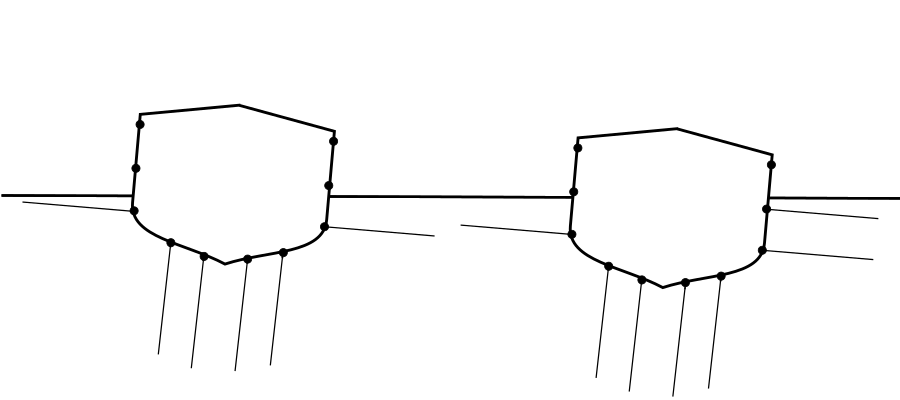
\includegraphics[width=110mm]{regular_grid}
\end{center}
\caption{Иллюстрация вычислительных артефактов за счет скачкообразного изменения гидродинамических сил при использовании регулярных сеток}
\label{regular_grid}
\end{figure}

Для устранения эффектов, указанных на \ref{regular_grid}, для интегрирования \eqref{F=integral} и \eqref{M=integral} используются квадратурные формулы типа Маркова с локально распределенными случайными узлами. Использование статичной или регулярной случайной сетки приводит к появлению нескомпенсированных сил, и, как следствие, самопроизвольному перемещению моделируемого судна. Для избавления от этого эффекта случайная сетка перестраивается на каждом шаге имитационного моделирования. Пример случайной сетки приведен на рис. \ref{monte_carlo}.

\begin{figure}[ht]
\begin{center}
\includegraphics[width=110mm]{monte_carlo}
\end{center}
\caption{Пример сетки с локально-распределенными случайными узлами}
\label{monte_carlo}
\end{figure}


%\section{Идентификация модели}

Cлучайное перестроение узлов может вносить в выражения \eqref{F=integral} и \eqref{M=integral} дополнительную вычислительную погрешность. Для оценки накапливаемой ошибки были проведены эксперименты по оценке чувствительности расчетных характеристик к количеству узлов сетки. На рис. \ref{drift} представлены фазовые портреты «численного дрейфа» (в плоскости $XY$) центра тяжести судна вокруг исходного положения (расчеты на тихой воде). На каждом графике показаны траектории движения центра тяжести судна для 10 запусков, каждый из которых длился 60 секунд.

Из рис. видно, что даже для достаточно грубых сеток погрешность не превышает 1 м, что является относительно небольшой величиной по сравнению с масштабами дрейфа под воздействием морского волнения.

\begin{figure}[ht]
\begin{center}
\includegraphics[width=140mm]{drift}
\end{center}
\caption{Фазовые портреты численного дрейфа судна в зависимости от количества точек $N$ }
\label{drift}
\end{figure}

Для идентификации модели рассмотрим процесс бортовой качки корабля на тихой воде.
В качестве испытательного образца возьмем судно класса "катер", который обладает следующими характеристиками:
\begin{description}
\item	Длина: $L = 40\ m$
\item	Ширина: $B = 7\ m$
\item	Вес: $D = 6 000 000\ N$
\end{description}

Для определения метацентрической высоты построим диаграмму статической остойчивости (ДСО) путем проведения виртуального кренования --- замера плеча восстанавливающего момента в зависимости от угла крена погруженного в воду судна. Результат кренования продемонстрирован на рис. \ref{stab}. Так как начальная метацентрическая высота равна дифференциалу ДСО в нулевой точке, то $h=1.03 м$

\begin{figure}[ht]
\begin{center}
\includegraphics[width=110mm]{stab}
\end{center}
\caption{Диаграмма статической остойчивости}
\label{stab}
\end{figure}

Определим период собственных бортовых колебаний согласно \citep{hanovich47} \eqref{roll_period}
\begin{equation}
	T_{roll} = \frac{0.80B}{\sqrt{h}} = 5.52\ s
	\label{roll_period}
\end{equation}

Момент инерции вокруг оси $X$ судна может быть приближенно вычислен по следующей формуле:
\begin{equation}
	I_{x} = (0.4B)^2 \frac{D}{g} \approx 4\ 700\ 000\ kg\cdot m^2
	\label{roll_torque}
\end{equation}



Момент сил сопротивления бортовым колебаниям может быть вычислен по формуле, полученной Бертеном \eqref{roll_torque}
\begin{equation}
	M_{roll} = kLB^4\dot{\alpha}^2
	\label{roll_torque}
\end{equation}

где $k$ лежит в диапазоне $10.0$ -- $20.0$. Для испытуемого судна возьмем значение $k$ равное $15.0$.

Составим дифференциальное уравнение бортовых колебаний судна:

\begin{equation}
	I_x \ddot{\alpha} + kLB^4\dot{\alpha}^2 + Dh \alpha = 0
	\label{roll_eq}
\end{equation}

Для идентификации модели корабль помещается на тихую воду с начальным креном $5$ градусов. Сравнение записи качки с результатом решения уравнение представлена на рис. \ref{expcmp}.

\begin{figure}[ht]
\begin{center}
\includegraphics[width=140mm]{expcmp}
\end{center}
\caption{Сравнение результатов численного эксперимента и решения уравнение бортовой качки}
\label{expcmp}
\end{figure}

Как видно и рисунка период и величина затухания бортовых колебаний соответствуют с высокой точностью, на основании чего можно сделать вывод, что численная модель движения судна позволяет воспроизводить эффекты частной модели.


%\include{ch2_03_math_ship_verify}
%
%\chapter{Программно-аппаратный комплекс виртуального полигона}

%\section{Состав и общая архитектура ПАК}

Разрабатываемый виртуальный полигон предназначен для выполнения имитационного моделирования 
динамики морских объектов под воздействием внешних возмущений. Как следствие, под задачей 
унификации в данном разделе понимается установление взаимосвязей общей (имитационной численной) 
модели динамики судна с «эталонными» моделями, повсеместно используемыми для расчета качки судна 
в оперативных условиях эксплуатации.

В отличие от традиционных моделей динамики судна (например, в форме уравнений движения), 
имитационная модель динамики судна представляет собой не только формализацию основных 
соотношений между входными и выходными данными, но и набор механизмов для проведения 
виртуальных экспериментов, которые должны:

\begin{enumerate}
\item	Обеспечивать настройку параметров имитационного моделирования в широких пределах.
\item	Создавать сценарии моделирования: параметры изменяются не только в начале, но и в процессе моделирования.
\item	Осуществлять интерактивную визуализацию процесса имитационного моделирования для осуществления качественного анализа явлений и отладки.
\item	Обеспечивать экспорт данных, в частности, в пакеты математического моделирования и проектирования.
\end{enumerate}

Таким образом, формой реализации имитационной модели является среда имитационного моделирования, которая содержит следующие специализированные и общие подсистемы:

\begin{enumerate}
	%--------------------------------
	% CORE
	%--------------------------------
	\item	Ядро (\frqt{Core}). В ядро подсистемы входят:
	\begin{enumerate}
		\item	Библиотека математики, которая включается как стандартные математические объекты, 
				такие как вектора, матрицы и кватернионы, так и более сложные, которые включают 
				такие объекты как видовые пирамиды (frustum), ограничивающие объемы (bounding sphere и bounding box).
		\item	Интерпретатор Lua, которые используется для конфигурирования 
				и управления виртуальным полигоном, 
				а также для поддержки подсистемы сценариев.
		\item 	Интерфейс операционной и файловой системы.
		\item	Система конфигурирования.
	\end{enumerate}
	%--------------------------------
	% GF
	%--------------------------------
	\item 	Библиотеки поддержки визуализации (\frqt{Graphic Factory}, собственная разработка), 
			которая независимо от используемого графического API обеспечивает:
			\begin{itemize}
			\item	Загрузку, обработку и сохранение трехмерных полигональных сеток в 
					формате собственной разработки ESX (Extensible Scene XML file). 
					В задачи обработки трехмерных полигональных сеток входят:
					\begin{itemize}
					\item	Разрезание, склеивание, оптимизация геометрии
					\item	Скелетная анимация
					\end{itemize}
			\item	Загрузку, обработку и сохранение двумерных изображений 
					в формате BMP, JPEG, TGA, PNG и другие. 
					Основан на использовании библиотеки FreeImage \citep{freeimage}.
			\item	Загрузку, обработку и сохранение файлов анимации в собственной формате 
					EAX (Extensible Animation XML-file). Файлы анимации могут быть использованы 
					для анимации визуализируемой сцены, анимацию камеры в демонстрационном режиме и др.
			\end{itemize}
	%--------------------------------
	% RS
	%--------------------------------
	\item	Графическая подсистема (\frqt{Reality Sequencer}, собственная разработка) 
			отвечает за подготовку сцены к отображению, построение теней, 
			расчета освещения, пост-обработки, а также отображение элементов пользовательского 
			интерфейса как в моно- так и стерео-режиме. В список графических объектов входят:
			\begin{enumerate}
			\item	Твердые объекты (Solids).
			\item	Водная поверхность (Water)\footnote{Так как генерация взволнованной поверхности 
					осуществляется с использованием графического ускорителя, генератор и визуализатор 
					водной поверхности для упрощения системы объединены в одну подсистему. 
					Обращаясь к графической подсистеме любая другая подсистема может задать 
					спектр волнения и запросить характеристики водной среды в любой точке и любой момент времени.}
			%\item	Объемные скалярные поля (Volume Scalar fields)
			\item	Отладочные линии (Debug lines).
			\item	Элементы пользовательского интерфейса и текст.
			\item	Источники света.
			\end{enumerate}
	%--------------------------------
	% SS
	%--------------------------------
	\item	Звуковая подсистема реализована с использованием \citep{fmod} предназначена для:
			\begin{itemize}
				\item	Воспроизведение Фонового стерео- и квадрофонического звука в 
						форматах Wave PCM, Vorbis OGG, MP3 и др.
				\item	Микширование с наложением эффектов окружения звуков, 
						позиционированных в пространстве, с учетом скорости 
						перемещения и позиции как звуков, так и слушателя.
			\end{itemize}

	%--------------------------------
	% PHYS
	%--------------------------------
	\item	Физическая подсистема реализована как интерфейс к физической 
			бибилиотеке Bullet \citep{bullet}. Реализация включает в себя:
			\begin{itemize}
				\item 	Твердые динамические тела
				\item 	Твердые статические тела
				\item 	Твердые кинематические тела
				\item 	Сочленения с шестью степенями свободы (6-DOF), 
						ограничениями (constarints), пружинами (springs) и моторам (motors).
			\end{itemize}
	
	%--------------------------------
	% XSB
	%--------------------------------
	\item
	Подсистема имитационного моделирования использует ("Extensible Sandbox") 
	представляет собой расширяемую библиотеку сущностей и параметров окружения, 
	в число которых входят такие классы сущностей как:
	\begin{enumerate}
		\item	\frqt{Таймер} --- запускает Lua-функцию в заданный момент времени
%		\item	Задача - запускает заданные определенным образом Lua-функции 
%				в заданные момент времени по определенному правилу.
		\item	\frqt{Корабль} --- реализует в себе модель распределения сил 
				и моментов, получает данные о море.
	\end{enumerate}
	Настраиваемым параметром окружения являются параметры волнения.
	Подсистема имитационного моделирования позволяет также добавлять 
			новые объекты и обеспечивает возможность их взаимодействия.
\end{enumerate}

%\begin{enumerate}
%\item	Подсистема имитационного использует язык высокого уровня для задания и изменения параметров моделирования, предварительной обработки результатов и формирования сценариев моделирования.
%\item	Модуль имитационного моделирования, в свою очередь состоит из:
%\begin{enumerate}
%\item	Генератора волнения. Генератор волнения формирует поле волнения по заданному спектру (например, Пирсона-Московица или JONSWAP) и передает необходимые для расчета значения в модель распределения сил и моментов.
%\item	Модели распределения сил и моментов. Она получает данные о поле волнения и, на основе поля волнения и данных о текущем положении судна, формирует набор сил и моментов, которые действуют по его корпусу в заданный момент времени.
%\item	Интегратора. Суммирует силы и моменты и решает задачу движения твердого тела под действием сил и моментов в заданный момент времени.
%\end{enumerate}
%\item 	Визуализатор отображает поле волнения и геометрическую модель судна, что позволяет визуально наблюдать процесс имитационного моделирования.
%\end{enumerate}

На рис. \ref{ship_dfd} показаны уровни абстракции в разработанной системе. 
Каждый элемент каждого уровня использует соседние элементы, а также все нижележащие элементы за исключением уровня операционной системы. Доступ к операционной системе разрешен лишь интерфейсу операционной и файловой системы. Такой подход облегчает дальнейшее портирование системы на другие платформы, а также упростить ряд типовых задач взаимодействия с операционной системой.

\begin{figure}[ht]
	\begin{center}
	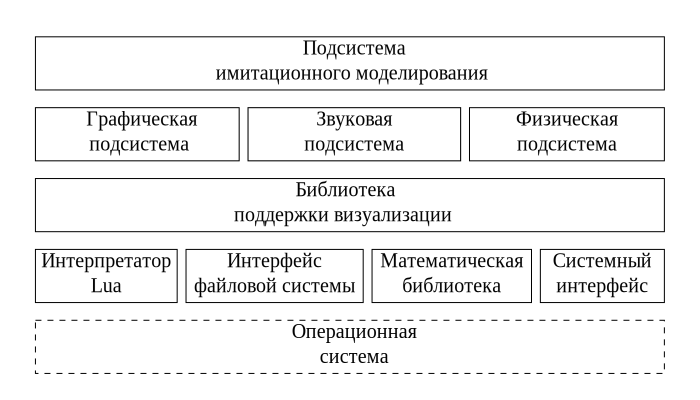
\includegraphics[width=150mm]{system_outline}
	\end{center}
	\caption{Уровни абстракции приложения}
	\label{ship_dfd}
\end{figure}

Следует отметить требования к аппаратному обеспечению. К ним относятся:
\begin{itemize}
	\item	Задачи визуализации и выполнения гидромеханических расчетов необходим 
	видео-ускоритель с поддержкой:
		\begin{itemize}
			\item	Архитектуры CUDA
			\item	Графической библиотеки OpenGL версии 3.3.
			\item	Модели шейдеров  vp40, fp40 --- поддержка расширений \linebreak
			$GL\_NV\_fragment\_program4$ и $GL\_NV\_vertex\_program4$.
		\end{itemize}
	\item	Для задач стерео-визуализации необходимо наличие:
		\begin{itemize}
			\item	Поддержки видео-ускорителем технологии OpenGL quad buffered stereo.
			\item	Наличие средств отображения стерео-контента, 
					таких как стерео-проекторы или стерео-мониторы.
		\end{itemize}	
	\item	Эффективное взаимодействие пользователя с ВП, обеспечивают комплекс устройст ввода, включающий как стандартные мышь и клавиатура, так и более развитые средства, такие как мыши с несколькими степенями свободы.
	\item 	Погружение в акустическую картину виртуального мира необходимо установка звуковой системы объемного звучания. 
\end{itemize}


%\include{ch3_02_scenario}
%\section{Подсистема моделирования}

Основная задачей подсистемы имитационного моделирования является управление сущностями (создание, обработка и уничтожение, а также их взаимодействие) и настройка параметров окружающей среды. Подсистема сценариев тесно связана с использованием языка программирования Lua \citep{lua}.

%------------------------------------------------------------------
%
%------------------------------------------------------------------

\subsection{Сущности и фабрика сущностей}

Для достижения высокого уровня абстракции и модульности в виртуальном полигоне применяются механизмы наследования и виртуальные функции. Полиморфизм, предоставляющий отложить выбор вызываемой функции (а как следствие --- поведение объектов) на период выполнения программы, обеспечивает повторное использование бинарного кода и его расширение.

Для обеспечения возможности определения типа создаваемого объекта в времени исполнения его необходимо указать. Механизм специализации типа создаваемого объекта называется фабрикой объектов \citep{alexandresku}.

Фабрика позволяет зарегистрировать фабричный метод (функцию создания объекта конкретного класса) и ассоциировать с ним некоторый дескриптор (например, константную строку). Следует отметить, что зарегистрировать фабричный метод можно не только на этапе компиляции, но и на этапе выполнения.

Создать объект заданного класса можно вызвав соответствующий метод фабрики класса и указав дескриптор.
Также, в фабричный метод можно передать дополнительные параметры создания объекта.

В данной реализации виртуального полигона все создаваемые объекты называются \frqt{сущностями} и наследуются от абстрактного класса $\tt entity$.

\begin{lstlisting}[caption={Декларация класса $\tt entity$}]
class entity {
public:
                  entity          ( uint id );
    virtual      ~entity          ( void ) {};
							
    virtual void  spawn           ( lua_State *L, int tidx ) = 0;
    virtual void  think           ( float dtime ) = 0;
    virtual int   command         ( const string &cmd, 
                                    lua_State *L ) = 0;
};
\end{lstlisting}

Сущность должна создаваться, существовать и при этом что-то делать, а также реагировать на внешние события.
В момент создания вызывается метод $\tt spawn$, в который передается указатель на виртуальную машину и индекс таблицы-дескриптора в стеке Lua. Это позволяет создавать объекты путем вызова методов на языке Lua.

На каждом шаге моделирования у каждой созданной сущности вызывается метод $\tt think$, в которые передается время прошедшее с предыдущего шага моделирования.

Для того чтобы взаимодействовать с сущностью используется метод $\tt command$, который можно рассматривать как \frqt{приказ}. В метод $\tt command$ передается строковая команда и указатель на виртуальную машину Lua, что позволяет через стек Lua передать любые параметры. Такой подход обеспечивает возможность отдачи приказов не только из C++ кода, но и из Lua кода.


Центральной компонентой системы имитационного моделирования является фабрика сущностей.
Интерфейс фабрики представлен ниже.

\begin{lstlisting}[caption={Интерфейс фабрики сущностей}]
class factory {
    public:
    factory     ( void );
    ~factory    ( void );

    typedef	entity	*(*create_func)	( uint id );

    void        register_class   ( const string &classname, 
                                   create_func create );
    uint        spawn_entity     ( const string &classname, 
                                   lua_State *L, int tidx );
    void        kill_entity      ( uint id );
    void        kill_all         ( void );
    entity    * get_entity       ( uint id );
    entity    * get_entity       ( const string &name );
};
\end{lstlisting}

Метод $\tt register\_class$ регистрирует класс сущностей, путем ассоциирования имени класса ($\tt classname$) и фабричного метода ($\tt create$).

Метод $\tt spawn\_entity$ порождает сущность класса $\tt classname$. 
Также в функцию передается указатель на виртуальную машину Lua и индекс таблицы-дескриптора, которая может быть использована для параметризации создаваемой сущности.
Метод возвращает уникальный индекс сущности, по которому в дальнейшем к сущности можно обратиться.

Метод $\tt kill\_entity$ --- уничтожает сущность с указанным индексом.

Метод $\tt kill\_all$ --- уничтожает все созданные сущности.

Метод $\tt get\_entity$ --- возвращает указатель на сущность по индексу или по имени.

На данный момент реализована следующая иерархия классов сущностей. См. рис.~\ref{entities}

\begin{figure}[ht]
\begin{center}
\includegraphics[width=110mm]{entities}
\end{center}
\caption{Диаграмма наследования сущностей}
\label{entities}
\end{figure}

%------------------------------------------------------------------
%
%------------------------------------------------------------------

\subsection{Lua API виртуального полигона}

Для обеспечения гибкости и универсальности виртуального полигона используется язык программирования Lua.
Такой подход позволяет создавать сценарии экспериментов \frqt{на ходу} не перезапуская виртуальный полигон.
Для обеспечения работы виртуального полигона, доступа к фабрике сущностей предусмотрены следующие Lua-функции:

\begin{itemize}
\item $\tt scenario.start$ --- запускает сценарий, которые задается 	
\item $\tt scenario.end$ --- завершает сценарий, виртуальный полигон переходит в 
режим ожидания. Никаких процессов моделирования не осуществляется.
\item $\tt scenario.spawn$ --- создает экземпляр сущности заданного класса. Аргументы функции: имя класса сущности и таблица-дескриптор. Возвращает индекс сущности.
\item $\tt scenario.kill$ --- уничтожает сущность с указанным именем или индексом.
\item $\tt scenario.kill\_all$ --- уничтожает все сущности.
\item $\tt scenario.command$ --- транслирует команду сущности заданной по имени или индексу.
\item $\tt scenario.time$ --- возвращает текущее глобальное модельное время.
\item $\tt scenario.set\_gravity$ --- устанавливает уровень гравитации.
\item $\tt scenario.set\_waving$ --- устанавливает параметры морского волнения:
	\begin{itemize}
	\item Частота пика спектра $\omega_{max}$.
	\item Параметр формы углового распределения $m$.
	\item Параметр узости спектра JONSWAP $\gamma$.
	\end{itemize}
\end{itemize}


%------------------------------------------------------------------
%
%------------------------------------------------------------------

\subsection{Объект \frqt{Таймер}}

Важной задачей в процессе моделирования является выполнение той или иной функции в заданный момент времени, или с постоянным интервалом. Для этого реализована сущность \frqt{Таймер}. При создании, таймер получает в качестве параметров:
\begin{itemize}
	\item	Интервал срабатывания --- временной интервал, через который будет вызываться Lua-функция. Если интервал равен $0$, то функция будет вызываться на каждом шаге моделирования.
	\item	Режим работы: однократное срабатывание или многократное.
	\item	Lua-функция для вызова\footnote{В языке Lua функции являются объектами первого класса, и могут быть переданы как параметр в функцию аналогично объекту любого другого типа \citep{implua}}.
\end{itemize}

Пример создания таймера на языке Lua представлен ниже:

\begin{lstlisting}[caption={Пример создания таймера}]
local id1 = scenario.spawn {
    classname   =   "timer";
    period      =   0.250;         
    once        =   false;      
    func        =   function () 
        print("timer function")
    end
}
\end{lstlisting}

Созданный таким образом таймер будет многократно с интервалом 250 мс выводить на консоль текст \frqt{timer function}.

Сам по себе объект таймер является достаточно примитивным и не очень удобным для выполнения различных задач. 
Поэтому для упрощения исследования динамики морских объектов была реализована система задач.

\subsubsection{Реализация системы задач на базе сущности \frqt{Таймер}}
Типовой эксперимент в численном исследовании динамики морского объекта заключается в следующем:
\begin{enumerate}
	\item	Создание судна и формирование параметров окружения 
			(данном случае параметров морского волнения).
	\item	Выполнение на каждом кадре моделирования некоторого действия, например удержание судна 
			в заданной точке.
	\item	Выполнение некоторого действия с заданным интервалом, например запись в журнал текущих							параметров судна
	\item	Уничтожение судна и сброс параметров морского волнения по прошествию некоторого времени. 
			Обычно эксперимент длится от 30 секунд, до 10 минут.
	\item	Вышеперечисленные действия повторяются либо для судна с другими параметрами 
			(например, с измененной нагрузкой или курсом), либо для морского волнения с другими параметрами (например, с другой частотой пика спектра или параметром формы углового распределения).
\end{enumerate}

Под задачей подразумевается совокупность функций, вызов которых должны быть осуществлен в определенные момент времени. В процессе проведения экспериментов были выявлены следующие требования к системе задач.
\begin{enumerate}
	\item Возможность запуска задачи в заданный момент времени.
	\item 	Возможность вызова функции в момент запуска задачи. 
	\item Возможность вызова функции в момент завершения задачи.
	\item Возможность вызова функции с определенным интервалом.
	\item Возможность вызова функции на каждом шаге моделирования.
	\item Возможность параллельного исполнения задач (функции являются атомарными).
	\item Возможность удобного составления расписания.
\end{enumerate}

Реализованная система задач работает следующим образом:
\begin{enumerate}
	\item 	Задаются функции $\tt init\_func$, $\tt term\_func$, $\tt frame\_func$, 
			$\tt tick\_func$? которые будут вызваны соответственно в момент создания задачи, 
			завершения задачи, на каждом шаге моделирования и с заданным интервалом 
			(на каждом \frqt{тике}).
	\item	Задаются время запуска задачи, время работы задачи и интервал между \frqt{тиками}.
	\item 	Создается таймер запуска задачи.
	\item 	В момент срабатывания таймера запуска задачи создается задача. 
			Таймер запуска задачи уничтожается.
	\item 	В момент создания задачи создаются три таймера, каждый из которых отвечает за:
	\begin{enumerate}
	\item	Вызов функции с заданным интервалом.
	\item	Вызов функции на каждом шаге моделирования.
	\item	Завершение задачи.
	\end{enumerate}	 
	\item 	После создания таймеров вызывается функция $\tt init\_func$.
	\item	По завершению задачи вызывается функция $\tt term\_func$ и все 
			таймеры созданные для этой задачи уничтожаются.
\end{enumerate}

Система задач предоставляет две функции:
\begin{itemize}
	\item	$\tt tasks.run()$ - непосредственный запуск задачи. 
			Принимает в качестве параметра Lua-таблицу --- 
			дескриптор задачи, в котором хранятся время выполнения задачи, 
			интервал между \frqt{тиками}, а также функции 
			$\tt init\_func$, $\tt term\_func$, $\tt frame\_func$ 
			и $\tt tick\_func$. Возвращает абсолютное время завершения задачи.
	\item	$\tt tasks.run_at()$ - отложенный запуск задачи. 	
			Принимает время запуска задачи и Lua-таблицу --- дескриптор задачи. 
			Возвращает абсолютное время завершения задачи.
\end{itemize}

Пример составления расписания задач представлен ниже:

\begin{lstlisting}[caption={Пример создания расписания задач}]
local tt1, tt2 = 0, 0;

for i=1, 10 do
  tt1 = tasks.run_at( tt1+1,  x_drift_task(i, 1) );
  tt1 = tasks.run_at( tt1+1,  x_drift_task(i, 2) );
  tt1 = tasks.run_at( tt1+1,  x_drift_task(i, 4) );
  tt1 = tasks.run_at( tt1+1,  x_drift_task(i, 8) );
end

for i=1, 16 do
  tt2 = tasks.run_at( tt2+1,  x_logging_task(i, 1) );
end
\end{lstlisting}

Вышепредставленный листинг демонстрирует создание расписания из 40 последовательно задач $\tt x\_drift\_task$ (функция, которая конструирует дескриптор задачи) и 16 последовательных задач 
$\tt x\_logging\_task$, которые будут выполняться параллельно.

Следует отметить, что система задач реализована полностью на языке Lua, затрагивать C++ код необходимости не было.

%------------------------------------------------------------------
%
%------------------------------------------------------------------

\subsection{Объект \frqt{Корабль}}




%\section{Графическая подсистема}

\subsection{Общая структура графической подсистемы}

Графическая подсистема логически разделена на два уровня абстракции:
\begin{itemize}
	\item	Драйвер (driver).
	\item	Сцена (scene).
\end{itemize}

Драйвер --- представляет собой слой абстракции от конкретного графического API.
Таким образом, это позволяет внедрять новые графические API не затрагивая сцену.
Основными сущностями драйвера, которыми он оперирует и предоставляет ну уровень выше --- сцене, являются:
\begin{itemize}
	\item	Эффект (Effect) --- представляет собой совокупность 
			состояний графического конвейера и набора из вершинного и пиксельного шейдера.
	\item	Вершинный буфер (Vertex buffer) --- представляет собой совокупность из набора массива вершин и массива индексов.
	\item	Текстура (Texture) --- двумерное (2D texture), трехмерное (Volume texture) или кубическое (Cube texture) изображение.
	\item	Внеэкранная поверхность (Render Target) --- может быть использована 
			как область, куда может осуществляться визуализация, а затем как двумерная текстура.
\end{itemize}


Как было отмечено выше графическая подсистема позволяет отображать следующие виды объектов:

\begin{itemize}
	\item	Твердые объекты (Solids).
	\item	Водная поверхность (Water).
	\item	Объемные скалярные поля (Volume Scalar fields).
	\item	Отладочные линии (Debug lines).
	\item	Элементы пользовательского интерфейса и текст.
	\item	Источники света.
\end{itemize}

Для отображения твердых объектов используется технология Deferred Shading \citep{stalker}, \citep{killzone}.
Для для закраски твердых объектов используется модель освещения Кука-Торренса, которая является физически обоснованной \citep{cook_torrance} и дает наиболее реалистичные блики \citep{ngan}.
Детальное описание техники визуализации твердых объектов, построения теней и расчета освещения представлено в статье \citep{bezgodov08}.
Пример построения теней представлен на рис.~\ref{shadows}.

\begin{figure}[ht]
\begin{center}
\includegraphics[width=150mm]{shadows}
\end{center}
\caption{Построение теней от элементов надстройки корабля}
\label{shadows}
\end{figure}



Для отображения элементов пользовательского интерфейса и текста используются списки наборы четырехугольников с наложенными текстурами.
Для отображения текста используются растровые шрифты, которые могут быть подготовлены из TrueType или OpenType шрифтов с использованием утилиты Bitmap Font Generator \citep{bmfont}.

Для отображения отладочной информации графическая система предоставляет функциональность по рендерингу трехмерных линий, 
а также следующих объектов, составляемых из линий:

\begin{itemize}
	\item	Стрелки (варьируются цвет, длина и форма наконечника)
	\item	Точки (изображаются как три взаимно-пересекающихся отрезка, варьируются размер и цвет)
	\item	Ориентированные по осям проволочный параллелепипед (варьируются размер и цвет)
\end{itemize}

Отладочные линии, а также их составные из линий объекты могут использованы для визуализации такой информации как:
\begin{itemize}
	\item	Силы и моменты действующие на судно.
	\item	Линии тока.
	\item	Траектории движения и графики.
\end{itemize}

На рис.~\ref{super_plot} представлен пример отладочной визуализации и текста.

\begin{figure}[ht]
\begin{center}
\includegraphics[width=110mm]{super_plot}
\end{center}
\caption{Отладочная визуализация и текст}
\label{super_plot}
\end{figure}

Для отображения трехмерных скалярных полей используется технология объемного рендеринга, которая 
заключается в трассировке луча в пространстве объемной текстуры и последующим накоплением 
значения трансфер-функции вычисленной для данной точки объема \citep{Engel01high-qualitypre-integrated}.
Пример объемного рендеринга на примере магнитных полей представлен на рис.~\ref{volume}

\begin{figure}[ht]
\begin{center}
\includegraphics[width=110mm]{volume}
\end{center}
\caption{Пример рендеринга скалярных полей}
\label{volume}
\end{figure}

\subsection{Морфологическое сглаживание степенчатости изображения}
В широкоэкранных системах ВР остро встает проблема «ступенчатости» изображений, которая обусловлена конечным размером пикселя. Например, для экрана системы ВР ЦСМВ СПбГУ ИТМО размер пикселя при разрешении 1920х1080 будет составлять около 2 мм, что визуально ощутимо на небольшом расстоянии от экрана. 

Для того чтобы избавиться от этого эффекта и сделать изображение более реалистичным используются специальные техники сглаживания.
На данный момент существует два наиболее часто используемых метода сглаживания, это избыточная выборка сглаживания (англ. Super Sampling anti-aliasing, SSAA) и множественная выборка сглаживания (англ. Multisample anti-aliasing, MSAA). Метод SSAA заключается в том, что вначале синтезируется изображение, в несколько раз превосходящее по размерам финального изображение, после чего это изображение сжимается до размеров финального, при этом происходит усреднение всех соседних пикселей. В результате работы SSAA получается наиболее качественное изображение, но данный метод крайне требователен к производительности системы и к её памяти, а в случае визуализации стереоизображения эти требования возрастают в два раза, что является мало приемлемым. Метод MSAA аналогичен SSAA, с той лишь разницей, что расчет цвета пикселя осуществляется один раз и записывается сразу в несколько суб-пикселей.

Следует отметить, что необходимость использования сглаживания и синтеза изображения высокого разрешения, а также синтез парных изображений (для создания эффекта стерео) ставит ограничение на возможность использования SSAA и MSAA, так как сильно возрастает объем памяти необходимый для буфера изображения. В связи с такими ограничениями было решено использовать метод морфологического сглаживания (англ. Morphological Antialiasing, MLAA)\citep{mlaa}. МLAA работает со сценами любой сложности и с любой техникой, фактически данный метод работает только с финальным изображением, он не настолько требователен к объему памяти как вышеперечисленные методы, а результат в большинстве случае не уступает результату работы метода SSAA. 

Данный метод заключается в нахождении \glqq L\grqq-образных форм на \frqt{ступенчатых} разрывах непрерывности и их размытии. Метод MLAA можно условно разделить на три этапа: 
\begin{enumerate}
\item	На этом этапе находятся все разрывы непрерывности в изображении, 
		точность на этом этапе можно повысить благодаря использованию Z-буфера. 
		На этом этапе можно применить любой метод нахождения разрывов непрерывностей 
		(граней, ребер) из области компьютерного зрения.
\item	На втором этапе рассчитывается длина найденных непрерывностей, это необходимо 
		для расчета уровня сглаживания пикселей. 
\item	На третьем этапе происходит поиск всех \glqq L\grqq-образных форм и их сглаживание.
\end{enumerate}

На рис.~\ref{mlaa} приведен пример синтезированного изображения без сглаживания и с использованием с MLAA.

\begin{figure}[ht]
\begin{center}
\includegraphics[width=140mm]{mlaa}
\end{center}
\caption{Результат применения морфологического сглаживания}
\label{mlaa}
\end{figure}





%---------------------------------------------------------------------------------
%	WATER RENDERING :
%---------------------------------------------------------------------------------

\subsection{Технология отображения морского волнения}

Для создания эффекта присутствия необходимо отображать визуально бесконечную водную поверхность простирающуюся о точки наблюдения до горизонта. Для визуализации безграничного моря используются две основные техники:
\begin{enumerate}
\item	Сетки в пространстве экрана (Screen space grids) \citep{projgrid}.
\item	Неравномерные, привязанные к камере сетки \cite{crysis}.
\end{enumerate}

В ходе работы были реализованы оба варианта визуализации водной поверхности. Вариант с использованием неравномерных сеток привязанных к камере оказался более стабильным и с небольшими изменениями используется как основной.
Для отображения используется сетка подготовленная особым образом. cм. рис.~\ref{sea_surface_twin}. Сетка имеет следующую структуру: 

\begin{itemize}
\item	А - \frqt{дно} - используется для маркировки буфера трафарета при отображении раздела сред; 
\item	B - \frqt{область волнения} - используется для отображения волн; 
\item	C - \frqt{область горизонта} - область, которая находится достаточно далеко от наблюдателя и видимой высотой волн можно пренебречь.
\end{itemize}

\begin{figure}[ht]
\begin{center}
\includegraphics[width=140mm]{sea_surface_twin}
\end{center}
\caption{Сетка для отображения морской поверхности. Слева – общая структура сетки, справа – сетка области интенсивного волнения. (обозначения – по тексту)}
\label{sea_surface_twin}
\end{figure}

Построение элементов сетки \frqt{A} и \frqt{С} --- тривиально. Построение области \frqt{A} осуществляется следующим образом:
\begin{enumerate}
	\item	Строится сетка размером состоящая из 16 квадратов.
	\item	Четыре центральных квадрата разбиваются еще на 4 квадрата каждый.
	\item	Шаг №2 повторяется 5-6 раз.
	\item 	К полученной сетке применяется алгоритм сглаживания полигональных сеток Катмулла-Кларка \citep{catmull_clark}.
\end{enumerate}

Полученная таким образом сетка обладает преимуществом перед сетками составленным из квадратных патчей, которое заключается в сглаживании границы перехода между более детальным и менее детальным участком сетки.

При визуализации моря, центр сетки всегда находится под или над камерой. Поворот камеры на ориентацию сетки в пространстве не влияет. Высота вершин в области «B» модифицируется вершинным шейдером на GPU в соответствии с моделью волнения. При этом, высота волн плавно уменьшается по мере увеличения расстояния от наблюдателя. Карта высот волн сгенерированная с использованием FFT на CUDA записывается в текстуру (этот процесс осуществляется полностью на GPU) и полученная текстура используется вершинным шейдером для модификации высоты вершин. Для эффекта отражения Френеля необходимо знать значение нормали в каждой точке. Для этого карта высот волн сэмплируется в нескольких точках и нормаль получается методом конечных разностей.


% ФРЕНЕЛЬ %

При закрашивании водной поверхности учитывается частичное отражение Френеля (только небо, которое задается панорамной текстурой), 
и частичное преломление с экспоненциальным затуханием по глубине. См. рис.~\ref{water_effects}.

\begin{figure}[ht]
\begin{center}
\includegraphics[width=140mm]{water_effects}
\end{center}
\caption{Визуализация поверхнсти воды: отражение Френеля (слева), экспоненциальное затухание с глубиной (справа).}
\label{water_effects}
\end{figure}


% РАЗДЕЛ СРЕД %

Следует отметить, что камера может находиться не только над водой, но и под водой, а также, на границе сред. Для корректного отображения границы сред используется следующая техника:
\begin{enumerate}
\item	При визуализации морской поверхности включается запись в буфер трафарета: каждый раз растеризуется треугольник значение соответствующего бита в буфере трафарета инвертируется. Таким образом, если пиксель находится внутри сетки, то значение в буфере трафарета будет равно 1, и 0 – если пиксель находится за пределами сетки.
\item	Для всех пикселей, для которых значение в буфере трафарета равно 1 применяется эффект затуманивания.
\end{enumerate}

Изображение полученное при позиционировании камеры на граница сред представлено на рис.~\ref{water_fog}.

\begin{figure}[ht]
\begin{center}
\includegraphics[width=140mm]{water_fog}
\end{center}
\caption{Визуализация границы сред}
\label{water_fog}
\end{figure}


% КОРАБЕЛЬНЫЕ ВОЛНЫ %

Дополнительным аспектом отображения визуальных свойств водной поверхности является воспроизведение расходящихся корабельных волн при движении плавучего морского объекта. Поскольку нелинейная задача расчета корабельных волн в полной постановке является существенно более ресурсоемкой по сравнению с моделью (??????), для создания визуального эффекта используется упрощенная модель, основанная на решении линейного уравнения колебаний на регулярной сетке:

\begin{equation}
	\frac{d^2U}{dt^2} = \frac{d^2U}{dx^2} +  \frac{d^2U}{dy^2}
\end{equation}

Начальное возмущение формируется в точке пересечения корпуса корабля и водной поверхности. Величина возмущения определяется в зависимости от относительной скорости поверхности корабля относительно воды. Уравнение решается на GPU с использованием библиотеки CUDA, результат расчета как набор значений в текстуре передается в вершинный шейдер и высота колебаний добавляется к высоте волн. В тех областях, где скорость частиц колеблющейся поверхности выше определенного значения, поверхность моря перекрашивается в белый цвет, что дает эффект пены. См. рис.~\ref{wakes}.

\begin{figure}[ht]
\begin{center}
\includegraphics[width=140mm]{wakes}
\end{center}
\caption{Корабельные волны)}
\label{wakes}
\end{figure}

Корабельные волны в данной реализации являются только визуальным эффектом и на ход моделирования поведения судна не влияют.






\chapter{Применение ВП для воспроизведения экстремальных ситуаций}

\section{Общий подход анализа резонансных явлений}

Для рассмотрения резонансных свойств судна на нерегулярном волнении воспользуемся функцию распределением Коши (или функцию отклика) в виде:

\begin{equation}
	R(\omega) = \frac{A \Delta \omega^2} {  (\Omega-\omega)^2 + \Delta \omega^2 } 
		 = \frac{A \left( \frac{\Omega}{Q} \right) ^2} {  (\Omega-\omega)^2 + \left( \frac{\Omega}{Q} \right) ^2 } 
\label{cauchy}
\end{equation}

$\omega$ --- частота, $\Omega_0$ --- резонансная частота, $A$ --- пиковая амплитуда, $\Delta \omega$ --- полоса пропускания, $Q$ --- добротность, величина, показывающая соотношение запасенной энергии к потерям энергии на сопротивление.

Примеры резонансных кривых представлены на рис.~\ref{rc}.

\begin{figure}[h!]
\begin{center}
\includegraphics[width=90mm]{resonance_curve}
\end{center}
\caption{Примеры резонансных кривых для разных параметров выражения \eqref{cauchy}}.
\end{figure}

Анализ резонансных явлений осуществляется путем аппроксимации экспериментальных данных функцией $R(\omega)$ методом наименьших квадратов. Обработка результатов и построение графиков осуществляется пакетом Scilab \citep{scilab}.


\section{Режим основного резонанса}

\subsection{Типовые аварии}


\subsection{Цель и постановка эксперимента}

\textbf{Условием} основного резонанса является совпадение частот собственных колебаний судна и частоты пика спектра волнения: $\omega_{roll} \approx \omega_{max}$.

\textbf{Целью} эксперимента является исследование влияние направленности волнения на возникновение резонанса и определение диапазона частот опасных для судна.

Для проведения эксперимента используется модель корабля класса \frqt{буксир} со следующими характеристиками:
\begin{itemize}
	\item	$L = 20\ \text{м}$
	\item	$B = 7\ \text{м}$
	\item	$T = 2\ \text{м}$
	\item	$D = 120\ 000\ \text{кг}$
\end{itemize}

Эксперимент состоит из следующих этапов:
\begin{enumerate}
	\item	Определение частот собственных колебаний судна 
			$\omega_{roll}$, $\omega_{pitch}$, $\omega_{heave}$ путем кренования на тихой воде.
	\item	Выбирается набор параметров внешних условий вида $(m, \omega_{max})$, для которых
			проводятся запись качки судна, в течении 120 секунд.
	\item	Этап №2	проводится для всех значений $m$ и $\omega_{max}$
	
			$m \in \left\lbrace 2,8,32,128,512 \right\rbrace$
			
			$\omega \in [0.8..3.0],\ \Delta\omega=0.1\ \text{рад/с}$ 

\end{enumerate}

\subsection{Анализ результатов эксперимента}

Согласно результатам эксперимента были получены следующие частоты собственных колебаний (временные диаграммы качки показаны на рис.~\ref{exp_rr_rolling}):
\begin{itemize}
	\item	$ \omega_{roll} = 1.75\ \text{рад/с}$
	\item	$ \omega_{pitch} = 2.15\ \text{рад/с}$
	\item	$ \omega_{heave} = 2.87\ \text{рад/с}$
\end{itemize}

\begin{figure}[ht]
	\begin{center}
	\includegraphics[width=120mm]{exp_rr/rolling}
	\includegraphics[width=120mm]{exp_rr/pitching}
	\includegraphics[width=120mm]{exp_rr/heaving}
	\end{center}
	\caption{Временные диаграммы бортовой, килевой и вертикальной качки}
	\label{exp_rr_rolling}
\end{figure}

Для всех параметров морского волнения определяется 10\%-ная обеспеченность (90\%-ная квантиль) модуля угла бортовой качки и делится на корень общей энергию волнения. График данного соотношения в зависимости от частоты пика спектра волнения и параметра формы углового распределения показан на рис.~\ref{rr:data} и рис.~\ref{rr:dataf} (аппроксимированные данные).

На основании аппроксимации можно сделать выводы:
\begin{enumerate}
	\item	Параметр формы углового распределения значительно влияет на установившуюся амплитуду колебаний судна.
	\item 	При увеличении значения формы углового распределения энергетические потери незначительно снижаются.
\end{enumerate}

\begin{sidewaysfigure}
	\includegraphics[width=230mm]{exp_rr/roll_resonance}
	\caption{Экспериментальные данные соотношения 10\%-ной обеспеченность модуля угла бортовой качки к энергии волнения.}
	\label{rr:data}
\end{sidewaysfigure}

\begin{sidewaysfigure}
	\includegraphics[width=230mm]{exp_rr/roll_resonance_f}
	\caption{Аппроксимация данных соотношения 10\%-ной обеспеченность модуля угла бортовой качки к энергии волнения и параметры функции отклика.}
	\label{rr:dataf}
\end{sidewaysfigure}

%\begin{figure}[ht]
%	\begin{center}
%	\includegraphics[width=100mm]{exp_rr/roll_resonance}
%	\includegraphics[width=100mm]{exp_rr/roll_resonance_f}
%	\end{center}
%	\caption{График соотношения 10\%-ной обеспеченность модуля угла бортовой качки к энергии волнения.}
%	\label{rr_res}
%\end{figure}

Как видно из графика пик резонанса приходится на диапазон частот 1.75-1.9, что приближенно соответствует собственной частоте бортовой качки судна.
\section{Режим параметрического резонанса (судно расположено лагом к волне)}

\subsection{Типовые аварии}


\subsection{Цель и постановка эксперимента}

\textbf{Условием} возникновение параметрического резонанса является периодическое изменение характеристик остойчивости судна (\frqt{валкость}), что, при совпадении частот изменения остойчивости судна и частоты собственных бортовых колебаний может привести к возникновению резонансу.
Изменение характеристик остойчивости судна может происходить при изменении осадки (которое может быть обусловлено вертикальной качкой). Если выполняется условие
$2 \omega_{roll} \approx \omega_{heave} \approx \omega_{max}$, то судно может попасть резонанса, что может привести к опасному крену.

\textbf{Целью} эксперимента является определение и сравнение опасных диапазонов частот морского волнения.

Для проведения эксперимента используется модель корабля класса \frqt{катер} со следующими характеристиками:
\begin{itemize}
	\item	$L = 40\ \text{м}$
	\item	$B = 12\ \text{м}$
	\item	$T = 3\ \text{м}$
	\item	$D = 600\ 000\ \text{кг}$
\end{itemize}

Эксперимент состоит из следующих этапов:
\begin{enumerate}
	\item	Определение частот собственных колебаний судна 
			$\omega_{roll}$, $\omega_{pitch}$, $\omega_{heave}$ путем кренования на тихой воде.
	\item	Выбирается набор частот пика спектра волнения $(m, \omega_{max})$, для которых
			проводятся запись качки судна, в течении 900 секунд.
	\item	Этап №2	проводится для всех значений $\omega_{max}$
			
			$\omega \in [0.8..3.0],\ \Delta\omega=0.05$ 

\end{enumerate}

\subsection{Анализ результатов эксперимента}

Согласно результатам эксперимента были получены следующие частоты собственных колебаний (временные диаграммы качки показаны на рис.~\ref{exp_pr_rolling_lag}):
\begin{itemize}
	\item	$ \omega_{roll} = 1.14 \text{с}^{-1}$
	\item	$ \omega_{pitch} = 3.25 \text{с}^{-1}$
	\item	$ \omega_{heave} = 2.36 \text{с}^{-1}$
\end{itemize}

\begin{figure}[ht]
	\begin{center}
	\includegraphics[width=120mm]{exp_pr_lag/rolling}
	\includegraphics[width=120mm]{exp_pr_lag/pitching}
	\includegraphics[width=120mm]{exp_pr_lag/heaving}
	\end{center}
	\caption{Временные диаграммы бортовой, килевой и вертикальной качки.}
	\label{exp_pr_rolling_lag}
\end{figure}

Для всех параметров морского волнения определяется 10\%-ная обеспеченность (90\%-ная квантиль) модуля угла бортовой качки и делится на корень общей энергии волнения. График данного соотношения (исходные результаты) в зависимости от частоты пика спектра волнения показан на рис.~\ref{exp_pr_rolling_resonance_lag}.

\begin{figure}[ht]
	\begin{center}
	\includegraphics[width=120mm]{exp_pr_lag/roll_resonance}
	\end{center}
	\caption{Временные диаграммы бортовой, килевой и вертикальной качки.}
	\label{exp_pr_rolling_resonance_lag}
\end{figure}

На графике присутствуют два вида резонанса:
\begin{itemize}
	\item	Основной --- приходится на частоты $1.0..1.5$.
	\item	Параметрический --- приходится на частоты $2.1..2.2$.
\end{itemize}


\section{Брочинг}

Брочинг --- явление потери управляемости при движении судна на попутных волнах, когда, подхваченное догоняющей волной, оно начинает двигаться со скоростью волны на ее переднем склоне и стремится развернуться к ней логом. Когда брочинг заканчивается полным разворотом судна, его крен за счет удара догоняющей волны и инерционного момента может достичь опасных пределов. Наибольшую опасность брочинг представляет для малых судов.

\subsection{Цель и постановка эксперимента}

\textbf{Условием} возникновения брочинга является:
\begin{itemize}
	\item	Движение судна в направлении распространения волн: $V=c$.
	\item	Длина волны ((соответствующая $\omega_{max}$)) находится в диапазоне от длины судна до удвоенной длины судна:
			: $L \leqslant c \leqslant 2L$.
	\item	Достаточно высокая степень регулярности волнения (зыбь): $\gamma > 10$.
\end{itemize}

\textbf{Целью} эксперимента является сбор статистики возникновения явления брочинга в одинаковых условиях (различие присутствует только в стохастических параметрах, таких как фазы гармоник морского волнения).

Для проведения используются следующие параметры волнения:
\begin{itemize}
	\item	$\omega_{max} = 1.2$
	\item	$\gamma = 20$
	\item	$m = 64$
\end{itemize}

Для проведения эксперимента используется модель судна класса \frqt{буксир} со следующими характеристиками:
\begin{itemize}
	\item	$L = 20\ m$
	\item	$B = 7\ m$
	\item	$T = 2\ m$
	\item	$D = 120\ 000\ kg$
\end{itemize}

Эксперимент состоит из следующих этапов:
\begin{enumerate}
	\item	Определение буксировочной диаграммы судна --- зависимости скорости судна от приложенной силы. 
			На основе данной диаграммы выбирается постоянная буксировочная сила. 
			Диаграмма строится следующим образом: на тихой воде к судну прикладывается фиксированная 
			сила с течении заданного промежутка времени 30 с (за это скорость для столь малого судна 
			должна установиться), после чего средняя скорость за последние 10 секунд 
			сопоставляется в выбранной буксировочной силой.
	\item	Проводится $N=200$ запусков (длительность $60 s$\footnote{60 секунд --- достаточное время развития явления брочинга для столь малого судна}) в одинаковых начальных условиях (различается лишь seed в генераторе случайных чисел \footnote{Используется вихрь Мерсенна \citep{mersenn_twister}})
\end{enumerate}


%----------------------------------------------------------------------

\subsection{Анализ результатов эксперимента}

Частоте волнения соответствует фазовая скорость $c = 8.167\ \text{м/с}$.
Согласно эксперименту по определению буксировочной силы, для достижения скорости $8.167\ \text{м/с}$ необходимо приложить силу равную $305\ \text{кН}$

\begin{figure}[ht]
	\begin{center}
	\includegraphics[width=130mm]{exp_broaching2/propulsion}
	\end{center}
	\caption{Диаграмма установившейся скорости и буксировочной силы}
	\label{tug_force}
\end{figure}

В ходе эксперимента были записаны все текущие параметры судна. На основе визуального анализа траектории были выделены следующие категории явления:

\begin{enumerate}
	\item	Присутствует значительное изменение курса с последующим восстановлением направление движения. 
			Явление может повториться вновь.
	\item	Изменение курса судна и отклонение и смещение судна от заданной траектории незначительно.
	\item	Крайне значительное изменение курса судна. Судно остается лагом к волне.
	\item	Значительное изменение курса судна.
	\item	Судно сохраняет общее направление движения, но периодически незначительно меняет курс.
\end{enumerate}

На рис.~\ref{all_tracks} представлены пять классов траекторий судна в режиме брочинга.
А на рис.~\ref{broaching11}, ~\ref{broaching12}, ~\ref{broaching13}, ~\ref{broaching14}, ~\ref{broaching15} --- подробные графики различных характеристик судна для наиболее типичных для каждого класса случаев.

\begin{sidewaysfigure}
	\begin{center}
	\includegraphics[width=210mm]{exp_broaching2/all_tracks}
	\end{center}
	\caption{Классы траекторий судна в режиме брочинга}
	\label{all_tracks}
\end{sidewaysfigure}



\begin{sidewaysfigure}
	\begin{center}	\includegraphics[width=210mm]{exp_broaching2/class_typical_1}	\end{center}
	\caption{Классы траектории I}	\label{broaching11}
\end{sidewaysfigure}

\begin{sidewaysfigure}
	\begin{center}	\includegraphics[width=210mm]{exp_broaching2/class_typical_2}	\end{center}
	\caption{Классы траектории II}	\label{broaching12}
\end{sidewaysfigure}

\begin{sidewaysfigure}
	\begin{center}	\includegraphics[width=210mm]{exp_broaching2/class_typical_3}	\end{center}
	\caption{Классы траектории III}	\label{broaching13}
\end{sidewaysfigure}

\begin{sidewaysfigure}
	\begin{center}	\includegraphics[width=210mm]{exp_broaching2/class_typical_4}	\end{center}
	\caption{Классы траектории IV}	\label{broaching14}
\end{sidewaysfigure}

\begin{sidewaysfigure}
	\begin{center}	\includegraphics[width=210mm]{exp_broaching2/class_typical_5}	\end{center}
	\caption{Классы траектории V}	\label{broaching15}
\end{sidewaysfigure}

Результаты эксперимента сведены в таблицу.~\ref{table_broaching}.

\begin{table}[h!]
\caption{Сводная таблица результатов проведения эксперимента}
\label{table_broaching}
\begin{center}

	%\rotatebox{90}{ %это обеспечивает поворот любого объекта
	\begin{tabular}{|c|ccccc|}
	\hline
	\rotatebox{90}{Класс траектории}	&	
	\rotatebox{90}{Отклонение от курса ($\phi_{max}$)}		&	
	\rotatebox{90}{Угол крена ($\theta_{max}$)}	&	
	\rotatebox{90}{Скорость ($V$)}	&	
	\rotatebox{90}{Угловая скорость ($\theta'_{max}$)}	&	
	\%	\\
	\hline
	I		&	70.63	&	25.92	&	7.84	&	0.18	&	23	\\
	II		&	68.00	&	25.87	&	7.95	&	0.13	&	10	\\
	III		&	101.73	&	42.38	&	7.96	&	0.24	&	22	\\	
	IV		&	77.91	&	39.18	&	8.02	&	0.21	&	41	\\
	V		&	58.54	&	19.23	&	8.74	&	0.13	&	4	\\
	\hline
	\end{tabular}
	%}
	
\end{center}
\end{table}

Потеря управляемости возникает в 90\% случаев.
Наиболее опасные варианты развития брочинга (максимальный крен $\theta_{max}$ достигает 40 градусов) 
соответствуют классам траекторий III и IV. Суммарная вероятность наиболее опасных вариантов развития события составляет 60\%.












%\chapter*{Заключение}
\addcontentsline{toc}{chapter}{Заключение}


В ходе выполнения диссертационного исследования автором лично был выполнен аналитический обзор в проблемной области диссертационной работы, проведена адаптация метода моделирования динамики судна на нерегулярном волнении к задаче формирования динамических сцен в ВП, проектирование, разработка и развертывание ВП, а также проведена серия экспериментов по воспроизведению таких экстремальных явлений, как основной и параметрический резонанс и брочинг. В диссертацию включены результаты, соответствующие личному участию автора, а именно:

\begin{itemize}

\item	развит метод численного моделирования экстремальной динамики МО с шестью степенями свободы на нерегулярном трехмерном волнении, основанный на интегрировании гидродинамических сил и моментов в нелинейной постановке на случайных сетках, допускающий интерактивное управление процессом вычислений на ВП;
\item	разработан метод формирования динамических сцен на основе численного моделирования динамики внешней среды и МО с учетом графических эффектов визуализации взволнованной поверхности моря и ее взаимодействия с корпусом объекта, адаптированный для применения в широкоэкранных системах ВР;
\item	разработана и детализирована архитектура ВП для изучения динамики МО в экстремальных условиях эксплуатации на основе модульного подхода к построению систем интерактивной визуализации;
\item		спроектирован и разработан программный комплекс ВП ShipX-DS, развернутый на инфраструктуре ЦСМВ СПбГУ ИТМО и продемонстрировавший свою работоспособность в ходе компьютерных экспериментов по исследованию экстремальной динамики МО в режиме основного и параметрического резонансов, а также в условиях брочинга.


%\item	развит метод численного моделирования экстремальной динамики МО с шестью степенями свободы на нерегулярном трехмерном волнении, основанный на интегрировании гидродинамических сил и моментов в нелинейной постановке на случайных сетках, допускающий интерактивное управление процессом вычислений в ВП;
%\item	разработан метод формирования динамических сцен на основе численного моделирования динамики внешней среды и МО, с учетом графических эффектов визуализации взволнованной поверхности моря и ее взаимодействия с корпусом объекта, адаптированный для применения в широкоэкранных системах ВР;
%\item	разработана и детализирована архитектура ВП для изучения динамики МО в экстремальных условиях эксплуатации на основе модульного подхода к построению систем интерактивной визуализации;
%\item	спроектирован и разработан программный комплекс ВП ShipX-DS, инсталлированный на инфраструктуре ЦСМВ СПбГУ ИТМО, и продемонстрировавший свою работоспособность в ходе компьютерных экспериментов по исследованию экстремальной динамики МО в режиме основного и параметрического резонансов, а также в условиях брочинга.

\end{itemize}
%\bibliographystyle{plain}
\addcontentsline{toc}{chapter}{Литература}
\bibliography{refs}


\end{document}


